% ****** Start of file apssamp.tex ******
%
%   This file is part of the APS files in the REVTeX 4.1 distribution.
%   Version 4.1r of REVTeX, August 2010
%
%   Copyright (c) 2009, 2010 The American Physical Society.
%
%   See the REVTeX 4 README file for restrictions and more information.
%
% TeX'ing this file requires that you have AMS-LaTeX 2.0 installed
% as well as the rest of the prerequisites for REVTeX 4.1
%
% See the REVTeX 4 README file
% It also requires running BibTeX. The commands are as follows:
%
%  1)  latex apssamp.tex
%  2)  bibtex apssamp
%  3)  latex apssamp.tex
%  4)  latex apssamp.tex
%
%\documentclass[reprint,superscriptaddress,showpacs,amsmath,amssymb,aps,prl,floatfix]{revtex4-1}
%\documentclass[superscriptaddress,showpacs,amsmath,amssymb,aps,prl,floatfix]{article}
\documentclass[aps,prl,superscriptaddress,showpacs,twocolumn,floatfix,amsmath,amssymb]{revtex4-1}

\usepackage{graphicx} % Include figure files
%\usepackage{dcolumn}  % Align table columns on decimal point
%\usepackage{bm}       % bold math
\usepackage{hyperref} % add hypertext capabilities
\usepackage[mathlines]{lineno} % Enable numbering of text and display math
\linenumbersep1mm
\linenumbers             % Commence numbering lines

\def\gtorder{\mathrel{\raise.3ex\hbox{$>$}\mkern-14mu
 \lower0.6ex\hbox{$\sim$}}}
\def\ltorder{\mathrel{\raise.3ex\hbox{$<$}\mkern-14mu
 \lower0.6ex\hbox{$\sim$}}}
\providecommand{\comment}[1]{{\bf \small \color{red} [#1]}}
\providecommand{\rcomment}[1]{{\bf \small \color{blue} [#1]}}

\begin{document}

%\title{Measurement of short-range correlations in nuclei at $x>1$ in inclusive quasi-elastic electron scattering}
\title{Search for three-nucleon short-range correlations in nuclei}

%%%%%%%%%%%%%%%%%%%%%%%%%%%%%%%%%%%%%%%%%%%%%%%%%%%%%

\newcommand*{\JLAB}{Thomas Jefferson National Accelerator Facility, Newport News, VA 23606}
\newcommand*{\TLV}{Tel Aviv University, Tel Aviv 69978, Israel}
\newcommand*{\MIT}{Massachusetts Institute of Technology, Cambridge, MA 02139}
\newcommand*{\KENT}{Kent State University, Kent, OH 44242}
\newcommand*{\DOMINION}{Old Dominion University, Norfolk, VA 23529}
\newcommand*{\CALIF}{California State University, Los Angeles, Los Angeles, CA 90032}
\newcommand*{\Hampton}{Hampton University, Hampton, VA 23668}
\newcommand*{\PENNSYLVANIA}{Pennsylvania State University, State College, PA 16801}
\newcommand*{\Paris}{Institut de Physique Nucl\'{e}aire (UMR 8608), CNRS/IN2P3 - Universit\'e Paris-Sud, F-91406 Orsay Cedex, France}
\newcommand*{\Syracuse}{Syracuse University, Syracuse, NY 13244}
\newcommand*{\Kentucky}{University of Kentucky, Lexington, KY 40506}
\newcommand*{\William}{College of William and Mary, Williamsburg, VA 23187}
\newcommand*{\Virginia}{University of Virginia, Charlottesville, VA 22904}
\newcommand*{\Halifax}{Saint Mary's University, Halifax, Nova Scotia, Canada}
\newcommand*{\Glasgow}{University of Glasgow, Glasgow G12 8QQ, Scotland, United Kingdom}
\newcommand*{\Temple}{Temple University, Philadelphia, PA 19122}
\newcommand*{\Argonne}{Physics Division, Argonne National Laboratory, Argonne, IL 60439}
\newcommand*{\China}{China Institute of Atomic Energy, Beijing, China}
\newcommand*{\NRCN}{Nuclear Research Center Negev, Beer-Sheva, Israel}
\newcommand*{\Catania}{Universita di Catania, Catania, Italy}
\newcommand*{\Dequense}{Duquesne University, Pittsburgh, PA 15282}
\newcommand*{\Pittsburgh}{Carnegie Mellon University, Pittsburgh, PA 15213}
\newcommand*{\LongwoodUniv}{Longwood University, Farmville, VA 23909}
\newcommand*{\Florida}{Florida International University, Miami, FL 33199}
\newcommand*{\Tallahassee}{Florida State University, Tallahassee, FL 32306}
\newcommand*{\INFN}{INFN, Sezione Sanit\`{a} and Istituto Superiore di Sanit\`{a}, 00161 Rome, Italy}
\newcommand*{\INFNBari}{INFN, Sezione di Bari and University of Bari, I-70126 Bari, Italy}
\newcommand*{\Ohio}{Ohio University, Athens, OH 45701}
\newcommand*{\Tennessee}{University of Tennessee, Knoxville, TN 37996}
\newcommand*{\Kharkov}{Kharkov Institute of Physics and Technology, Kharkov 61108, Ukraine}
\newcommand*{\LOSALAMOS}{Los Alamos National Laboratory, Los Alamos, NM 87545}
\newcommand*{\Duke}{Duke University, Durham, NC 27708}
\newcommand*{\Texas}{University of Texas, Houston, TX 77030}
\newcommand*{\Seoul}{Seoul National University, Seoul, Korea}
\newcommand*{\Indiana}{Indiana University, Bloomington, IN 47405}
\newcommand*{\Hampshire}{University of New Hampshire, Durham, NH 03824}
\newcommand*{\Blacksburg}{Virginia Polytechnic Inst. and State Univ., Blacksburg, VA 24061}
\newcommand*{\France}{Universit\'e Blaise Pascal/IN2P3, F-63177 Aubi\`ere, France}
\newcommand*{\Mississippi}{Mississippi State University, Mississippi State, MS 39762}
\newcommand*{\Austin}{The University of Texas at Austin, Austin, Texas 78712}
\newcommand*{\Norfolk}{Norfolk State University, Norfolk, VA 23504}
\newcommand*{\Lanzhou}{Lanzhou University, Lanzhou, China}
\newcommand*{\Hebrew}{Racah Institute of Physics, Hebrew University of Jerusalem, Jerusalem, Israel}
\newcommand*{\Rutgers}{Rutgers, The State University of New Jersey, Piscataway, NJ 08855}
\newcommand*{\Yerevan}{Yerevan Physics Institute, Yerevan 375036, Armenia}
\newcommand*{\Ljubljana}{University of Ljubljana, Ljubljana, Slovenia}
\newcommand*{\Michigan}{Northern Michigan University, Marquette, MI 49855}
\newcommand*{\Hefei}{University of Science and Technology, Hefei, China}	
\newcommand*{\Jozef}{Jozef Stefan Institute, Ljubljana, Slovenia}
\newcommand*{\Ecole}{CEA Saclay, F-91191 Gif-sur-Yvette, France}
\newcommand*{\Massachusetts}{University of Massachusetts, Amherst, MA 01006}

\author{Z. Ye}
\affiliation{\Argonne}
\affiliation{\Virginia}
\affiliation{\Duke}
\author{P. Solvignon}
\affiliation{\Hampshire}
\affiliation{\JLAB}
\author{D. Nguyen}
\affiliation{\Virginia}
\author{P. Aguilera}
\affiliation{\Paris}
\author{Z. Ahmed}
\affiliation{\Syracuse}
\author{H. Albataineh}
\affiliation{\DOMINION}
\author{K. Allada}
\affiliation{\JLAB}
\author{B. Anderson}
\affiliation{\KENT}
\author{D. Anez}
\affiliation{\Halifax}	
\author{K. Aniol}
\affiliation{\CALIF}
\author{J. Annand}
\affiliation{\Glasgow}
\author{J. Arrington}
\affiliation{\Argonne}
\author{T. Averett}
\affiliation{\William}
\author{H. Baghdasaryan}
\affiliation{\Virginia}
\author{X. Bai}
\affiliation{\China}
\author{A. Beck}
\affiliation{\NRCN}	
\author{S. Beck}
\affiliation{\NRCN}	
\author{V. Bellini}
\affiliation{\Catania}
\author{F. Benmokhtar}
\affiliation{\Dequense}
\author{A. Camsonne}
\affiliation{\JLAB}
\author{C. Chen}
\affiliation{\Hampton}
\author{J.-P. Chen}
\affiliation{\JLAB}
\author{K. Chirapatpimol}
\affiliation{\Virginia}
\author{E. Cisbani}
\affiliation{\INFN}
\author{M.~M. Dalton}
\affiliation{\Virginia}
\affiliation{\JLAB}
\author{A. Daniel}
\affiliation{\Ohio}
\author{D. Day}
\affiliation{\Virginia}
\author{W. Deconinck}
\affiliation{\MIT}
\author{M. Defurne}
\affiliation{\Ecole}	
\author{D. Flay}
\affiliation{\Temple}
\author{N. Fomin}
\affiliation{\Tennessee}
\author{M. Friend}
\affiliation{\Pittsburgh}
\author{S. Frullani}
\affiliation{\INFN}
\author{E. Fuchey}
\affiliation{\Temple}
\author{F. Garibaldi}
\affiliation{\INFN}
\author{D. Gaskell}
\affiliation{\JLAB}
\author{S. Gilad}
\affiliation{\MIT}
\author{R. Gilman}
\affiliation{\Rutgers}
\author{S. Glamazdin}
\affiliation{\Kharkov}
\author{C. Gu}
\affiliation{\Virginia}
\author{P. Gu\`eye}
\affiliation{\Hampton}
\author{C. Hanretty}
\affiliation{\Virginia}
\author{J.-O. Hansen}
\affiliation{\JLAB}
\author{M. Hashemi Shabestari}
\affiliation{\Virginia}
\author{O. Hen}
\affiliation{\TLV}
\author{D.~W. Higinbotham}
\affiliation{\JLAB}
\author{M. Huang}
\affiliation{\Duke}
\author{S. Iqbal}
\affiliation{\CALIF}
\author{G. Jin}
\affiliation{\Virginia}
\author{N. Kalantarians}
\affiliation{\Virginia}
\author{H. Kang}
\affiliation{\Seoul}
\author{A. Kelleher}
\affiliation{\MIT}
\author{I. Korover}
\affiliation{\TLV}
\author{J. LeRose}
\affiliation{\JLAB}
\author{J. Leckey}
\affiliation{\Indiana}	
\author{R. Lindgren}
\affiliation{\Virginia}
\author{E. Long}
\affiliation{\KENT}
\author{J. Mammei}
\affiliation{\Blacksburg}
\author{D. J. Margaziotis}
\affiliation{\CALIF}
\author{P. Markowitz}
\affiliation{\Florida}
\author{D. Meekins}
\affiliation{\JLAB}
\author{Z. Meziani}
\affiliation{\Temple}
\author{R. Michaels}
\affiliation{\JLAB}
\author{M. Mihovilovic}
\affiliation{\Jozef}
\author{N. Muangma}
\affiliation{\MIT}
\author{C. Munoz Camacho}
\affiliation{\France}
\author{B. Norum}
\affiliation{\Virginia}
\author{Nuruzzaman}
\affiliation{\Mississippi}
\author{K. Pan}
\affiliation{\MIT}
\author{S. Phillips}
\affiliation{\Hampshire}
\author{E. Piasetzky}
\affiliation{\TLV}
\author{I. Pomerantz}
\affiliation{\TLV}
\affiliation{\Austin}
\author{M. Posik}
\affiliation{\Temple}
\author{V. Punjabi}
\affiliation{\Norfolk}	
\author{X. Qian}
\affiliation{\Duke}	
\author{Y. Qiang}
\affiliation{\JLAB}
\author{X. Qiu}
\affiliation{\Lanzhou}
\author{P.~E. Reimer}
\affiliation{\Argonne}
\author{A. Rakhman}
\affiliation{\Syracuse}
\author{S. Riordan}
\affiliation{\Virginia}
\affiliation{\Massachusetts}
\author{G. Ron}
\affiliation{\Hebrew}
\author{O. Rondon-Aramayo}
\affiliation{\Virginia}
\author{A. Saha}
\thanks{deceased}
\affiliation{\JLAB}
\author{L. Selvy}
\affiliation{\KENT}
\author{A. Shahinyan}
\affiliation{\Yerevan}
\author{R. Shneor}
\affiliation{\TLV}
\author{S. Sirca}
\affiliation{\Ljubljana}
\author{K. Slifer}
\affiliation{\Hampshire}
\author{N. Sparveris}
\affiliation{\Temple}	
\author{R. Subedi}
\affiliation{\Virginia}
\author{V. Sulkosky}
\affiliation{\MIT}
\author{D. Wang}
\affiliation{\Virginia}
\author{J.~W. Watson}
\affiliation{\KENT}
\author{L.~B. Weinstein}
\affiliation{\DOMINION}
\author{B. Wojtsekhowski}
\affiliation{\JLAB}
\author{S.~A. Wood}
\affiliation{\JLAB}
\author{I. Yaron}
\affiliation{\TLV}
\author{X. Zhan}
\affiliation{\Argonne}
\author{J. Zhang}
\affiliation{\JLAB}
\author{Y.~W. Zhang}
\affiliation{\Rutgers}
\author{B. Zhao}
\affiliation{\William}
\author{X. Zheng}
\affiliation{\Virginia}
\author{P. Zhu}
\affiliation{\Hefei}
\author{R. Zielinski}
\affiliation{\Hampshire}	

\collaboration{The Jefferson Lab Hall A Collaboration}


%%%%%%%%%%%%%%%%%%%%%%%%%%%%%%%%%%%%%%%%%%%%%%%%%%%%%

\date{\today}

%\begin{linenomath}
\begin{abstract}

We present new data probing short-range correlations (SRCs) in nuclei through the measurement of electron scattering off high-momentum nucleons in
light nuclei. The inclusive cross section ratios of $^4$He/$^3$He and $^{12}$C/$^3$He are observed to be both $x$ and $Q^2$ independent
for $1.5 < x <2$, confirming the previously observed dominance of two-nucleon short-range correlations. The cross section ratios for
$x > 2$ do not agree with an earlier measurement which suggested that three-nucleon correlations dominated the interaction in this $Q^2$ range.
While 3N-SRCs may have an important contribution, these data suggest that they cannot be isolated in the same simple fashion as 2N-SRCs.

\end{abstract}
%\end{linenomath}

\pacs{13.60.Hb, 25.10.+s, 25.30.Fj}
\maketitle

%%%%%%%%%%%%%%%%%%%%%%%%%%%%%%%%%%%%%%%%%%%%%%%%%%%%%
%introduction
%% review

Understanding the complex structure of the nucleus remains one of the major uncompleted tasks in nuclear
physics, and significant questions remain about the high-momentum components of the nuclear wavefunction.
This is an important component of nuclear structure that goes beyond the shell model description. Mean field
calculations~\cite{DeForest1983} do not include these high-momentum components, and so typically overpredict
the cross section for proton knock-out reactions below the Fermi momentum~\cite{VanDerSteenhoven1988547,
Lapikas1993297, Kelly:1996hd}.

%Without the inclusion of these high-momentum components, the mean-field calculation using the distorted wave impulse
%approximation~\cite{DeForest1983}  overestimates the nuclear strength which had been observed by many proton knock-out
%experiments~\cite{VanDerSteenhoven1988547, Lapikas1993297, Kelly:1996hd}.

In the dense and energetic environment of the nucleus, nucleons have a significant probability of
interacting at distances $\le$1~fm, even in light nuclei~\cite{carlson14,lu13}. Protons and neutrons
interacting through the strong, short-distance components of the NN interaction give rise to pairs of
nucleons with large momenta. These high-momentum pairs, referred to as short-range correlations (SRCs), are
the primary source of high-momenta in nuclei~\cite{Frankfurt1981215, SLAC_Measurement_PRC.48.2451,
src_john}, well above the typical scale of the Fermi momentum ($k_F \approx 300$~MeV/c) associated with the
shell model picture of nuclear structure. For momenta below $k_F$, we observed shell-model behavior which is
strongly $A$ dependent, while two-body physics dominates above $k_F$, yielding a universal
structure for all nuclei that is driven by the details of the NN interaction~\cite{RevModPhys.80.189,
PhysRevC.53.1689, wiringa14}.

In inclusive electron scattering, the kinematics can be used to select scattering from high-momentum
nucleons. The electron transfers energy, $\nu$, and momentum, $\vec{q}$, to the struck nucleon by exchanging
a virtual photon with four momentum transfer $q^2 = - Q^{2} = \nu^{2}-|\vec{q}|^{2}$. It is useful in this
case to define the kinematic variable $x = Q^2/(2M_p\nu)$, where $M_p$ is the mass of the proton. Elastic
scattering from a stationary proton corresponds to $x=1$, while inelastic scattering must occur at $x<1$. In
a nucleus, the momentum of the nucleon yields a broad quasielastic peak centered near $x=1$. Scattering at
$x>1$ is beyond the kinematic threshold for scattering from a free nucleon and so must involve more than one
nucleon. At values of $x$ slightly greater than unity, scattering can occur either from nucleons with the
modest momenta expected from the mean field, or from high-momentum nucleons associated with SRCs. As $x$
increases, larger initial momenta are required until scattering from nucleons below the Fermi
momentum is kinematically forbidden, isolating scattering from high-momentum nucleons associated with
SRCs~\cite{RevModPhys.80.189, PhysRevC.53.1689, src_john, egiyan2003}.

Because the momentum distribution of the nucleus is not a physical observable, one cannot directly extract
and study its high-momentum component. One can, however, test the idea of a universal structure of the
high-momentum components by comparing scattering from different nuclei at kinematics which require that the
struck nucleon have a large initial momentum~\cite{RevModPhys.80.189}. Previous measurements at SLAC and
Jefferson Lab revealed a universal form to the high-momentum distributions of the struck
nucleons~\cite{SLAC_Measurement_PRC.48.2451, egiyan2003, PhysRevLett.96.082501, fomin2012, src_john,
arrington99, arrington01}. In these experiments, the cross section ratios for inclusive scattering from
heavy nuclei to the deuteron were shown to scale, i.e. be independent of $x$ and $Q^2$, for $x \gtorder 1.5$
and $Q^2 \gtorder 1.5$~GeV$^2$, corresponding to scattering from nucleons with momenta above 300 MeV/c.
Other measurements have demonstrated that these high-momentum components are dominated by high-momentum n-p
pairs~\cite{aclander99, tang03, Subedi13062008, korover2014, hen14_science, piasetzky06}, meaning that the high-momentum
components in all nuclei have a deuteron-like structure. While final-state interactions (FSI)
decrease with increasing $Q^2$ in inclusive scattering, FSI between nucleons in the correlated pair may not
disappear. It is typically assumed that the FSI are identical for the deuteron and the deuteron-like pair in
heavier nuclei, and thus cancel in these ratios~\cite{RevModPhys.80.189, src_john}.

This approach can be extended to look for universal behavior arising from 3N-SRCs by examining scattering at
$x>2$ (beyond the kinematic limit for scattering from a deuteron). Within the simple SRC
model~\cite{Frankfurt1981215}, the cross section is composed of scattering from one-body, two-body,
etc... configurations, with the one-body (shell-model) contributions dominating at $x \approx 1$, while
2N-SRCs (3N-SRCs) dominate as $x \to 2 (3)$. Taking ratios of heavier nuclei to $^3$He allows a similar
examination of the target ratios for $x>2$, where the simple SRC model predicts a universal behavior
associated with three-nucleon SRCs (3N-SRCs) - configurations where three nucleons have large relative
momenta but little total momentum. 3N-SRCs could come from either three-nucleon forces or successive hard
two-nucleon interactions. The first such measurement~\cite{PhysRevLett.96.082501} observed $x$-independent
ratios for $x > 2.25$. This was interpreted as a result of 3N-SRCs dominance in this region.
However the ratios were extracted at relatively small $Q^2$, and the $Q^2$ dependence was not measured. A
later experiment~\cite{fomin2012} at higher $Q^2$ yielded $^4$He/$^3$He ratios that were significantly
larger. Consequently, the question of whether 3N-SRC contributions have been cleanly identified and observed
to dominate at some large momentum scale is as yet unanswered.

% JRA: Some of this may be better/more concise than bit above.
%
%The first evidence of SRC in inclusive scattering was revealed by the SLAC data~\cite{SLAC_Measurement_PRC.48.2451} with $a_2(A)$ exhibiting a
%plateau between $x\sim1.5$ and $x\sim2$, where 2N-SRC is expected to dominate. A recent measurement from the CLAS data in Hall B at
%JLab~\cite{PhysRevLett.96.082501} also reported the 2N-SRC plateau in the $a_3(A)$ distribution. The latest measurement from the E02-019
%experiment in Hall C at JLab with better precision and a wider range of nuclei, and both $a_2(A)$ and $a_3(A)$ show clear 2N-SRC
%plateau~\cite{fomin2012}. In the $x>2$ region, while the CLAS data claimed a second plateau at $x>2$ in the
%$\sigma_{^{4}He}/\sigma_{^{3}He}$ ratio, E02-019 sees, despite the large error bars, clearly a rise in the $a_3(A)$ distribution. It should be
%noted that both experiments reported data at very different $Q^{2}$ and the kinematical requirement in performing a clean measurement of 3N-SRC is
%not yet well understood.


%The interaction between the virtual photon and the nucleon provides an unique probe to study the nucleon's initial state, e.g., the momentum distribution which is correlated to the scaling function~\cite{West1975263,day_arns, PhysRevC.41.R2474, Boffi19931,RevModPhys.80.189}:
%\begin{equation}
%F(y) = 2\pi\int_{|y|}^{\infty}n(p_{0})\cdot p_{0}dp_{0},
%	\label{fy_mom_eq}
%	\end{equation} 
%	where $n(p_{0})$ is the momentum distribution of the nucleon with the initial momentum $p_{0}$. $y$ is the solution of $M_{A}+\nu = \sqrt{M^{2}+|\vec{q}|^{2}+y^{2}+2y|\vec{q}|}+\sqrt{M_{A-1}^{2}+y^{2}}$ where $M$, $M_{A}$ and $M_{A}$ are the masses of the nucleon, target nucleus A and the (A-1) recoil system, respectively. $F(y)$ can be directly extracted from the experimental QE inclusive cross section:
%	\begin{equation}
%	F(y)=\frac{d^{3}\sigma_{EX}}{dE' d\Omega } \frac{1}{Z\sigma_{p}+N\sigma_{n}} \frac{q}{\sqrt{M^{2}+(y+q)^{2}}},
%	\label{fy_scaling_eq2}
%	\end{equation}
%	where $\sigma_{p}$ and $\sigma_{n}$ are the electron-proton and electron-neutron cross section, respectively.


%Compared with the electron elastic scattering process which is well peaked at $x=Q^{2}/2Mv=1$ (M is the proton mass), the QE process yields a much
%broader peaks at $x=1$ due to the Fermi motion of the nucleon inside the nucleus. By measuring the inclusive QE cross section at $x>1$ with
%$Q^{2}>1~GeV^{2}$, one can carefully map out the SRC in different nuclei by taking the ratio of the cross section per nucleon of the heavy nucleus,
%$A$, to the light nucleus, e.g. deuteron or $\mathrm{^{3}He}$:
%\begin{equation}
%a_{2}(A) = \frac{\sigma_{A}(x,Q^{2})/A}{\sigma_{D}(x,Q^{2})/2},~~~  a_3(A) = \frac{\sigma_{A}(x,Q^{2})/A}{\sigma_{^{3}He}(x,Q^{2})/3},
%\end{equation}



%%{\bf (talk about Doug and Or's Analysis, Phys.Rev.Lett. 114 (2015) 16, 169201, when we discuss our new results)}



%%%%%%%%%%%%%%%%%%%%%%%%%%%%%%%%%%%%%%%%%%%%%%%%%%%%%
Understanding the complex structure of the nucleus remains one of the major uncompleted tasks in nuclear physics, and significant questions remain about the high-momentum components of the nuclear wave-function. This important aspect of nuclear structure is not described by the shell model description. This high-momentum strength appears at low momenta in Mean field calculations~\cite{DeForest1983} which subsequently over predict the cross section for proton knock-out reactions below the Fermi momentum~\cite{VanDerSteenhoven1988547, Lapikas1993297, Kelly:1996hd}.

%This is an important component of nuclear structure that goes beyond the shell model description. Mean field
%calculations~\cite{DeForest1983} do not include these high-momentum components, and so typically overpredict
%the cross section for proton knock-out reactions below the Fermi momentum~\cite{VanDerSteenhoven1988547,
%Lapikas1993297, Kelly:1996hd}.

%Without the inclusion of these high-momentum components, the mean-field calculation using the distorted wave impulse
%approximation~\cite{DeForest1983}  overestimates the nuclear strength which had been observed by many proton knock-out
%experiments~\cite{VanDerSteenhoven1988547, Lapikas1993297, Kelly:1996hd}.

In the dense and energetic environment of the nucleus, nucleons have a significant probability of
interacting at distances $\le$1~fm, even in light nuclei~\cite{carlson14,lu13}. Protons and neutrons
interacting through the strong, short-distance part of the NN interaction give rise to pairs of
nucleons with large momenta. These high-momentum pairs, referred to as short-range correlations (SRCs), are
the primary source of high-momenta in nuclei~\cite{Frankfurt1981215, SLAC_Measurement_PRC.48.2451,
src_john}, well above the typical scale of the Fermi momentum ($k_F \approx 300$~MeV/c) associated with the
shell model picture of nuclear structure. For momenta below $k_F$, we observe shell-model behavior which is
strongly $A$ dependent, while two-body physics dominates above $k_F$ resulting in a universal
structure for all nuclei that is steered by the details of the NN interaction~\cite{RevModPhys.80.189,
PhysRevC.53.1689, wiringa14}.

In the case of inclusive electron scattering it is possible  through kinematics, as follows, to isolate events in which the electron interacts with  high-momentum nucleons. The electron transfers energy, $\nu$, and momentum, $\vec{q}$, to the struck nucleon by exchanging
a virtual photon with four momentum transfer $q^2 = - Q^{2} = \nu^{2}-|\vec{q}|^{2}$. It is useful in this
case to define the kinematic variable $x = Q^2/(2M_p\nu)$, where $M_p$ is the mass of the proton. Elastic
scattering from a stationary proton corresponds to $x=1$, while inelastic scattering must occur at $x<1$. In
a nucleus, the momentum of the nucleon produces a broad quasielastic peak centered near $x=1$. 
%Scattering at
%$x>1$ is beyond the kinematic threshold for scattering from a free nucleon and so must involve more than one
%nucleon. At values of $x$ slightly greater than unity, scattering can occur either from nucleons with the
%modest momenta expected from the mean field, or from high-momentum nucleons associated with SRCs.
Scattering at $x>1$ is beyond the kinematic threshold for scattering from a free nucleon. At values of $x$ slightly greater than unity, scattering can occur either from nucleons with the modest momenta expected from the mean field, or from high-momentum nucleons associated with SRCs. As $x$
increases, larger initial momenta are required until scattering from nucleons below the Fermi
momentum is kinematically forbidden, isolating scattering from high-momentum nucleons associated with
SRCs~\cite{RevModPhys.80.189, PhysRevC.53.1689, src_john, egiyan2003}.

Because the momentum distribution of the nucleus is not a physical observable, one cannot directly extract
and study its high-momentum component. One can, however, test the idea of a universal structure of the
high-momentum components by comparing scattering from different nuclei at kinematics which require that the
struck nucleon have a large initial momentum~\cite{RevModPhys.80.189}. Previous measurements at SLAC and
Jefferson Lab revealed a universal form to the high-momentum distributions of the struck
nucleons~\cite{SLAC_Measurement_PRC.48.2451, egiyan2003, PhysRevLett.96.082501, fomin2012, src_john,
arrington99, arrington01}. In these experiments, the cross section ratios for inclusive scattering from
heavy nuclei to the deuteron were shown to scale, i.e. be independent of $x$ and $Q^2$, for $x \gtorder 1.5$
and $Q^2 \gtorder 1.5$~GeV$^2$, corresponding to scattering from nucleons with momenta above 300 MeV/c.
Other measurements have demonstrated that these high-momentum components are dominated by high-momentum n-p
pairs~\cite{aclander99, tang03, Subedi13062008, korover2014, hen14_science, piasetzky06}, meaning that the high-momentum
components in all nuclei have a deuteron-like structure. While final-state interactions (FSI)
decrease with increasing $Q^2$ in inclusive scattering, FSI between nucleons in the correlated pair may not
disappear. It is typically assumed that the FSI are identical for the deuteron and the deuteron-like pair in
heavier nuclei, and thus cancel in these ratios~\cite{RevModPhys.80.189, src_john}.

This approach can be extended to look for universal behavior arising from 3N-SRCs by examining scattering at
$x>2$ (beyond the kinematic limit for scattering from a deuteron). Within the simple SRC
model~\cite{Frankfurt1981215}, the cross section is composed of scattering from one-body, two-body,
etc... configurations, with the one-body (shell-model) contributions dominating at $x \approx 1$, while
2N-SRCs (3N-SRCs) dominate as $x \to 2 (3)$. Taking ratios of heavier nuclei to $^3$He allows a similar
examination of the target ratios for $x>2$, where the simple SRC model predicts a universal behavior
associated with three-nucleon SRCs (3N-SRCs) - configurations where three nucleons have large relative
momenta but little total momentum. 3N-SRCs could come from either three-nucleon forces or multiple hard
two-nucleon interactions. The first such measurement~\cite{PhysRevLett.96.082501} observed $x$-independent
ratios for $x > 2.25$. This was interpreted as a result of 3N-SRCs dominance in this region.
However the ratios were extracted at relatively small $Q^2$, and the $Q^2$ dependence was not measured. In the experiment of Ref.~\cite{fomin2012}, at higher $Q^2$, the $^4$He/$^3$He ratios  were significantly
larger. Consequently, the question of whether 3N-SRC contributions have been cleanly identified and observed
to dominate at some large momentum scale is as yet unanswered.

% JRA: Some of this may be better/more concise than bit above.
%
%The first evidence of SRC in inclusive scattering was revealed by the SLAC data~\cite{SLAC_Measurement_PRC.48.2451} with $a_2(A)$ exhibiting a
%plateau between $x\sim1.5$ and $x\sim2$, where 2N-SRC is expected to dominate. A recent measurement from the CLAS data in Hall B at
%JLab~\cite{PhysRevLett.96.082501} also reported the 2N-SRC plateau in the $a_3(A)$ distribution. The latest measurement from the E02-019
%experiment in Hall C at JLab with better precision and a wider range of nuclei, and both $a_2(A)$ and $a_3(A)$ show clear 2N-SRC
%plateau~\cite{fomin2012}. In the $x>2$ region, while the CLAS data claimed a second plateau at $x>2$ in the
%$\sigma_{^{4}He}/\sigma_{^{3}He}$ ratio, E02-019 sees, despite the large error bars, clearly a rise in the $a_3(A)$ distribution. It should be
%noted that both experiments reported data at very different $Q^{2}$ and the kinematical requirement in performing a clean measurement of 3N-SRC is
%not yet well understood.


%The interaction between the virtual photon and the nucleon provides an unique probe to study the nucleon's initial state, e.g., the momentum distribution which is correlated to the scaling function~\cite{West1975263,day_arns, PhysRevC.41.R2474, Boffi19931,RevModPhys.80.189}:
%\begin{equation}
%F(y) = 2\pi\int_{|y|}^{\infty}n(p_{0})\cdot p_{0}dp_{0},
%	\label{fy_mom_eq}
%	\end{equation} 
%	where $n(p_{0})$ is the momentum distribution of the nucleon with the initial momentum $p_{0}$. $y$ is the solution of $M_{A}+\nu = \sqrt{M^{2}+|\vec{q}|^{2}+y^{2}+2y|\vec{q}|}+\sqrt{M_{A-1}^{2}+y^{2}}$ where $M$, $M_{A}$ and $M_{A}$ are the masses of the nucleon, target nucleus A and the (A-1) recoil system, respectively. $F(y)$ can be directly extracted from the experimental QE inclusive cross section:
%	\begin{equation}
%	F(y)=\frac{d^{3}\sigma_{EX}}{dE' d\Omega } \frac{1}{Z\sigma_{p}+N\sigma_{n}} \frac{q}{\sqrt{M^{2}+(y+q)^{2}}},
%	\label{fy_scaling_eq2}
%	\end{equation}
%	where $\sigma_{p}$ and $\sigma_{n}$ are the electron-proton and electron-neutron cross section, respectively.


%Compared with the electron elastic scattering process which is well peaked at $x=Q^{2}/2Mv=1$ (M is the proton mass), the QE process yields a much
%broader peaks at $x=1$ due to the Fermi motion of the nucleon inside the nucleus. By measuring the inclusive QE cross section at $x>1$ with
%$Q^{2}>1~GeV^{2}$, one can carefully map out the SRC in different nuclei by taking the ratio of the cross section per nucleon of the heavy nucleus,
%$A$, to the light nucleus, e.g. deuteron or $\mathrm{^{3}He}$:
%\begin{equation}
%a_{2}(A) = \frac{\sigma_{A}(x,Q^{2})/A}{\sigma_{D}(x,Q^{2})/2},~~~  a_3(A) = \frac{\sigma_{A}(x,Q^{2})/A}{\sigma_{^{3}He}(x,Q^{2})/3},
%\end{equation}



%%{\bf (talk about Doug and Or's Analysis, Phys.Rev.Lett. 114 (2015) 16, 169201, when we discuss our new results)}


%%%%%%%%%%%%%%%%%%%%%%%%%%%%%%%%%%%%%%%%%%%%%%%%%%%%%
%experiment
%
The new JLab experiment, E08-014, was carried out in Hall A in 2011~\cite{e08014_pr} and focused on the measurements of inclusive cross sections at large $x$ with more statistics and better precision. An high intensity electron beam with a constant energy of $3.356~\mathrm{GeV}$ was employed to strick on a fixed target, and the scattered electrons were simultaneously detected by two identical High-Resolution Spectrometers (HRSs)~\cite{halla_nim}. Each spectrometer consist of a pair of vertical drift chambers (VDCs) for particle tracking, two scintillator planes for triggering and timing measurements, and a gas \v{C}erenkov counter and two layers of lead-glass calorimeters for particle identification. Three 20~cm long cryogenic targets, the liquid $\mathrm{^{2}D}$ , the $\mathrm{^{3}He}$ gas and the $\mathrm{^{4}He}$ gas, were measured, in addition to $\mathrm{^{12}C}$, $\mathrm{^{40}Ca}$ and $\mathrm{^{48}Ca}$. The spectrometers were positioned at $\theta_{0}=21^\circ$, $23^\circ$, $25^\circ$, and $28^\circ$ with total of 9 different central momentum settings, which includes the $\mathrm{Q^{2}}$ range from 1.1~$\mathrm{(GeV/c)^{2}}$ to 2.5~$\mathrm{(GeV/c)^{2}}$ and covers QE region up to $x_{bj}\sim 3$. The detailed description of the experiment and the data analysis can be found in Ref.~\cite{zye_thesis}.

% PID cuts and efficiencies
The electrons were identified by cutting on the calbirated signals of the \v{C}erenkov detector after the alignment of its ten ADC spectra. Additional cuts were applied on the calorimeters signals, including the energy sum normalized by the particle momentum, as well as a graphic cut on the two-dimensional histogram of the first layer's energy vs. the second layer's energy. The efficiencies of these selections are both above 99\% while the pion to electron ratio was estimated to be better than $\mathrm{10^{-4}}$ level due to the low pion production under our kinematic regions. The trigger efficiencies and the detection efficiencies of the \v{C}erenkov detector and calorimeters were carefully evaluated and the results are very close to 100\%.  We only kept events with one-track during the tracking reconstruction since the zero-track and multi-track events were less than 1\%.. 

% Acceptance
The scattered electron's initial momentum, in-plan and out-of-plan angles and its vertex position on the target can be reconstructed with the optics matrices of the HRSs and the tracking information from the VDCs. The optics matrices have been well extracted by many previous Hall A experiments and it were also optimized using the new calibration data taken during our experiment with a 30~cm long optics target composed of 7 carbon foils. The uncertainty from the optics reconstruction is believed to be better than $99\%$~\cite{halla_nim}. We cut on the central region of these reconstructed quantities to choose the best HRS acceptance and ran a Monte Carlo (MC) simulation of the HRSs~\cite{zye_thesis} to correct for the residual acceptance effect which is learnt to be well controlled. (Note: should we discuss the HRS-R Q3 issue and also its uncertainty of Dp correction?)

%targets
For the cryogenic targets, we removed the contaminated events from electrons scattering off the end-cups of the target cells by applying a cut on the reconstructed vertex position of the scattered electron on the target. A dummy target of two thin aluminum foils with 20~cm apart was used to evaluate the level of residual contamination after the cut. With the precise optics reconstruction, a cut of $\pm 7~cm$ at the center part of the target is able to remove $>99.9\%$ of the events from target end-cups.

One of the largest sources of systematic uncertainty come from the non-uniform target densities of $\mathrm{^{2}D}$, $\mathrm{^{3}He}$ and $\mathrm{^{4}He}$ due to the not well distributed coolant flow and the high beam current from $40~mu\mathrm{A}$ up to $120~mu\mathrm{A}$.  We took the boiling study data on these target with varying beam currents, and extrapolated the density profiles when the beam was off and normalized the distribution to the values obtained during the target installation. For safety, we assigned 5\% uncertainty of the target density for each cryogenic target. 

(FIX-HERE: Discuss more about the systematic uncertainties from different sources and make a table).

The cross sections were extracted by binning the data in $x$. A yield ratio method was developed to apply all necessary corrections only on the MC data until the MC yield converges to the experimental yield in the same x bin. The experimental yield for the $ith$ x bin is defined as:
\begin{equation}
Y^{i}_{EX} = \frac{N^{i}_{EX}}{N_{e}},
	\end{equation}
	where $N^{i}_{EX}$ is the number of scattered electrons within the bin after all event selections and acceptance cuts, and $N_{e}$ is the total number of incoming electrons hit on the target. The MC yield can be written as:
	\begin{equation}
	Y^{i}_{MC} = \epsilon_{eff} \cdot \eta_{tg}\cdot \frac{\Delta E'_{MC}\Delta \Omega_{MC}} {N_{MC}^{gen}}\cdot\sum_{j\in i}\sigma^{rad}_{model}(E_{j},E'_{j},\theta_{j}) .
	\label{eqymc}
	\end{equation}
	where $\epsilon_{eff}$ is the product of efficiencies from varied sources. $\eta_{tg}$ denotes the areal density of the scattering centers calculated from the target thickness, $\eta_{tg}=\rho\cdot l \cdot N_{A}/A$ where $N_{A}$ is the Avogadro's number. The target density has been corrected with the boiling effect. $\Delta E'_{MC}$ and $\Delta\Omega_{MC}$ are the momentum and solid angle overages of the HRS in the simulation which were chose to be slighly larger than the actuall ranges, and $N_{MC}^{gen}$ is the total number of generated MC events within the ranges. The terms in $\sum_{j\in i}$ represent that within the $ith$ x-bin, the $jth$ electron is first weighed by the radiated cross section calculated with the incoming beam energy $E_{j}$, outgoing momentum $E'_{j}$ and angle $\theta_{j}$ and then summurized. A cross section model was developed based on the $F(y)$ scaling and the peaking-approximation method was used to calculate the radiation effect~\cite{zye_thesis}. 

	The experimental cross section for the $ith$ x-bin is then given by:
	\begin{equation}
	\sigma_{EX}(E, E'_{i},\theta_{0}) = \frac{Y^{i}_{EX}}{Y^{i}_{MC}}\cdot\sigma_{model}(E, E'_{i},\theta_{0}),
	\end{equation}
	where $E$ is the beam energy fixed at 3.356 GeV, $\theta_{0}$ is the central scattering angle, $E'_{i}$, the scattered energy, is calculated based on $x_{i}$, and $\sigma_{model}(E, E'_{i},\theta_{0})$ is the cross section of the bin calculated from the model with the radiation effect corrected.  In this method, the bin-centering correction was automatically applied for choosing the center of the x-bin. The cross sections of different targets were extracted with exactly the same bins and the same acceptance cuts. Their statistical and systematic errors were individually calculated before taking the cross section ratio.

    Add more about analysis

%%%%%%%%%%%%%%%%%%%%%%%%%%%%%%%%%%%%%%%%%%%%%%%%%%%%%
The results reported here are from JLab experiment E08-014~\cite{e08014_pr}, which focused on precise
measurements of the $x$ and $Q^2$ dependence of the A/$^3$He cross section ratios at large $x$. A $3.356$~GeV
electron beam with currents ranging from 40 to 120 $\mu$A impinged on nuclear targets, and scattered
electrons were detected in two nearly identical High-Resolution Spectrometers (HRSs)~\cite{halla_nim}. Data
were taken on six targets: three 20-cm cryogenic targets (liquid $^2$H and gaseous $^3$He and $^4$He) and
thin foils of $\mathrm{^{12}C}$, $\mathrm{^{40}Ca}$ and $\mathrm{^{48}Ca}$. We focus here on the results from
the light nuclei, $A \leq 12$, which were taken to examine the 3N-SRC region, while the Calcium data were
taken to examine the isospin dependence in the 2N-SRC kinematics.

Each HRS consists of a pair of vertical drift chambers (VDCs) for particle tracking, two scintillator planes
for triggering and timing measurements, and a gas \v{C}erenkov counter and two layers of lead-glass
calorimeters for particle identification~\cite{halla_nim}. Scattering was measured at $\theta=21^\circ$,
$23^\circ$, $25^\circ$, and $28^\circ$, covering a $Q^2$ range of 1.3--2.2~GeV$^2$. A detailed description
of the experiment and data analysis can be found in Ref.~\cite{zye_thesis}.


% PID cuts and efficiencies

The data analysis is relatively straightforward, as the inclusive scattering at $x>1$ yields low rates and a
small pion background. The trigger and tracking inefficiencies are small and applied as a correction to the
measured yield. Electrons are identified by applying cuts on the signals from both the \v{C}erenkov detector
and the calorimeters. The cuts yield $>99$\% electron efficiency with negligible pion contamination. The
overall dead-time of the data acquisition system (DAQ) was evaluated on a run-by-run bases. To ensure a
well-understood acceptance, the solid angle and momentum acceptance were limited to high-acceptance regions
and a model of the HRSs~\cite{zye_thesis} was used to apply acceptance corrections.

The scattered electron momentum, in-plane and out-of-plane angles, and vertex position at the target can be
reconstructed from the VDC tracking information using the optics matrices determined in earlier experiments.
For the right HRS, the third quadrupole was unable to run at its full current, and so data were taken in a
modified tune with at 15\% reduction in its field. Optics data were taken to correct for the modified
tune. Many of the systematic uncertainties in the spectrometers are correlated, so we took the
conservative approach of applying these uncertainties to the combined result from the HRS-L and HRS-R data.

%targets

The cryogenic targets have a large background from scattering in the cell walls. We apply a $\pm 7$~cm
cut around the center of the target, removing $>99.9\%$ of the events from target endcap
scattering, as determined from measurements on empty target cells. One of the largest contributions to the
systematic uncertainty comes from target density reduction due to heating of the $^2$H, $^3$He, and $^4$He
targets because of the high-current electron beam. We made dedicated measurements over a range of
beam currents and used the variation of the yield to measure the current dependence of the target density.
The effect was large and varied with the position along the target, and the measurements were used to
determine the density loss and thus the effective target thicknesses of the measurement. Since much 
of the model dependence will be target independent, a conservative 5\% normalization uncertainty was applied
on the ratio of cryotargets to account for target density uncertainties.

%We assigned a conservative uncertainty of 5\% on the target density for each cryogenic target, but due to the
%fact that much of the model dependence will be target independent, take a 5\% combined normalization uncertain
%on the ratio of cryotargets.

The measured events, corrected for inefficiencies and normalized to the integrated luminosity, were binned
in $x$ and compared to the simulated yield. The simulation uses a $y$-scaling cross section
model~\cite{day_arns, arrington99} with radiative corrections applied using the peaking
approximation~\cite{zye_thesis, stein75}. Coulomb corrections are applied within an improved effective
momentum approximation~\cite{aste05}, and are 2\% or smaller for all data presented here.  The combined 
systematic uncertainty, neglecting the normalization uncertainty due to target thickness uncertainty,
is XX-YY\%, and is generally the largest contribution to the uncertainties in the ratios except at larger
$x$ values where the statistical uncertainty becomes larger.

%all targets except $^{40}$Ca and $^{48}$Ca, where the corrections are 5--6\% for the largest scattering angles. For each $x$ bin,
%the ratio of experimental to Monte Carlo yield is applied as a correction to the cross section model at that $x$ value to extract the cross section.


%The experimental cross section for the $ith$ bin is then given by:
%	\begin{equation}
%	\sigma_{EX}(E, E'_{i},\theta_{0}) = \frac{Y^{i}_{EX}}{Y^{i}_{MC}}\cdot\sigma_{model}(E, E'_{i},\theta_{0}),
%	\end{equation}
%where $E$ is the beam energy fixed at 3.356 GeV, $\theta_{0}$ is the central scattering angle, $E'_{i}$, the scattered energy, is calculated based on $x_{i}$, and $\sigma_{model}(E, E'_{i},\theta_{0})$ is the cross section of the bin calculated from the model with the radiation effect corrected.  In this method, the bin-centering correction was automatically applied for choosing the center of the x-bin. The cross sections of different targets were extracted with exactly the same bins and the same acceptance cuts. Their statistical and systematic errors were individually calculated before taking the cross section ratio.
%
%{\bf Talk about isoscalar correction not being apply because of the np dominance (JRA: Not till ratios at the earliest). Coulomb correction.}



%%%%%%%%%%%%%%%%%%%%%%%%%%%%%%%%%%%%%%%%%%%%%%%%%%%%%
%results	
%%%%%%%%%%%%%%%%%%%%%%%%%%%%%%%%%%%%%%%%%%%%%%%%%%%%%
%%results

                \begin{figure}[!ht]
		\begin{center}
		  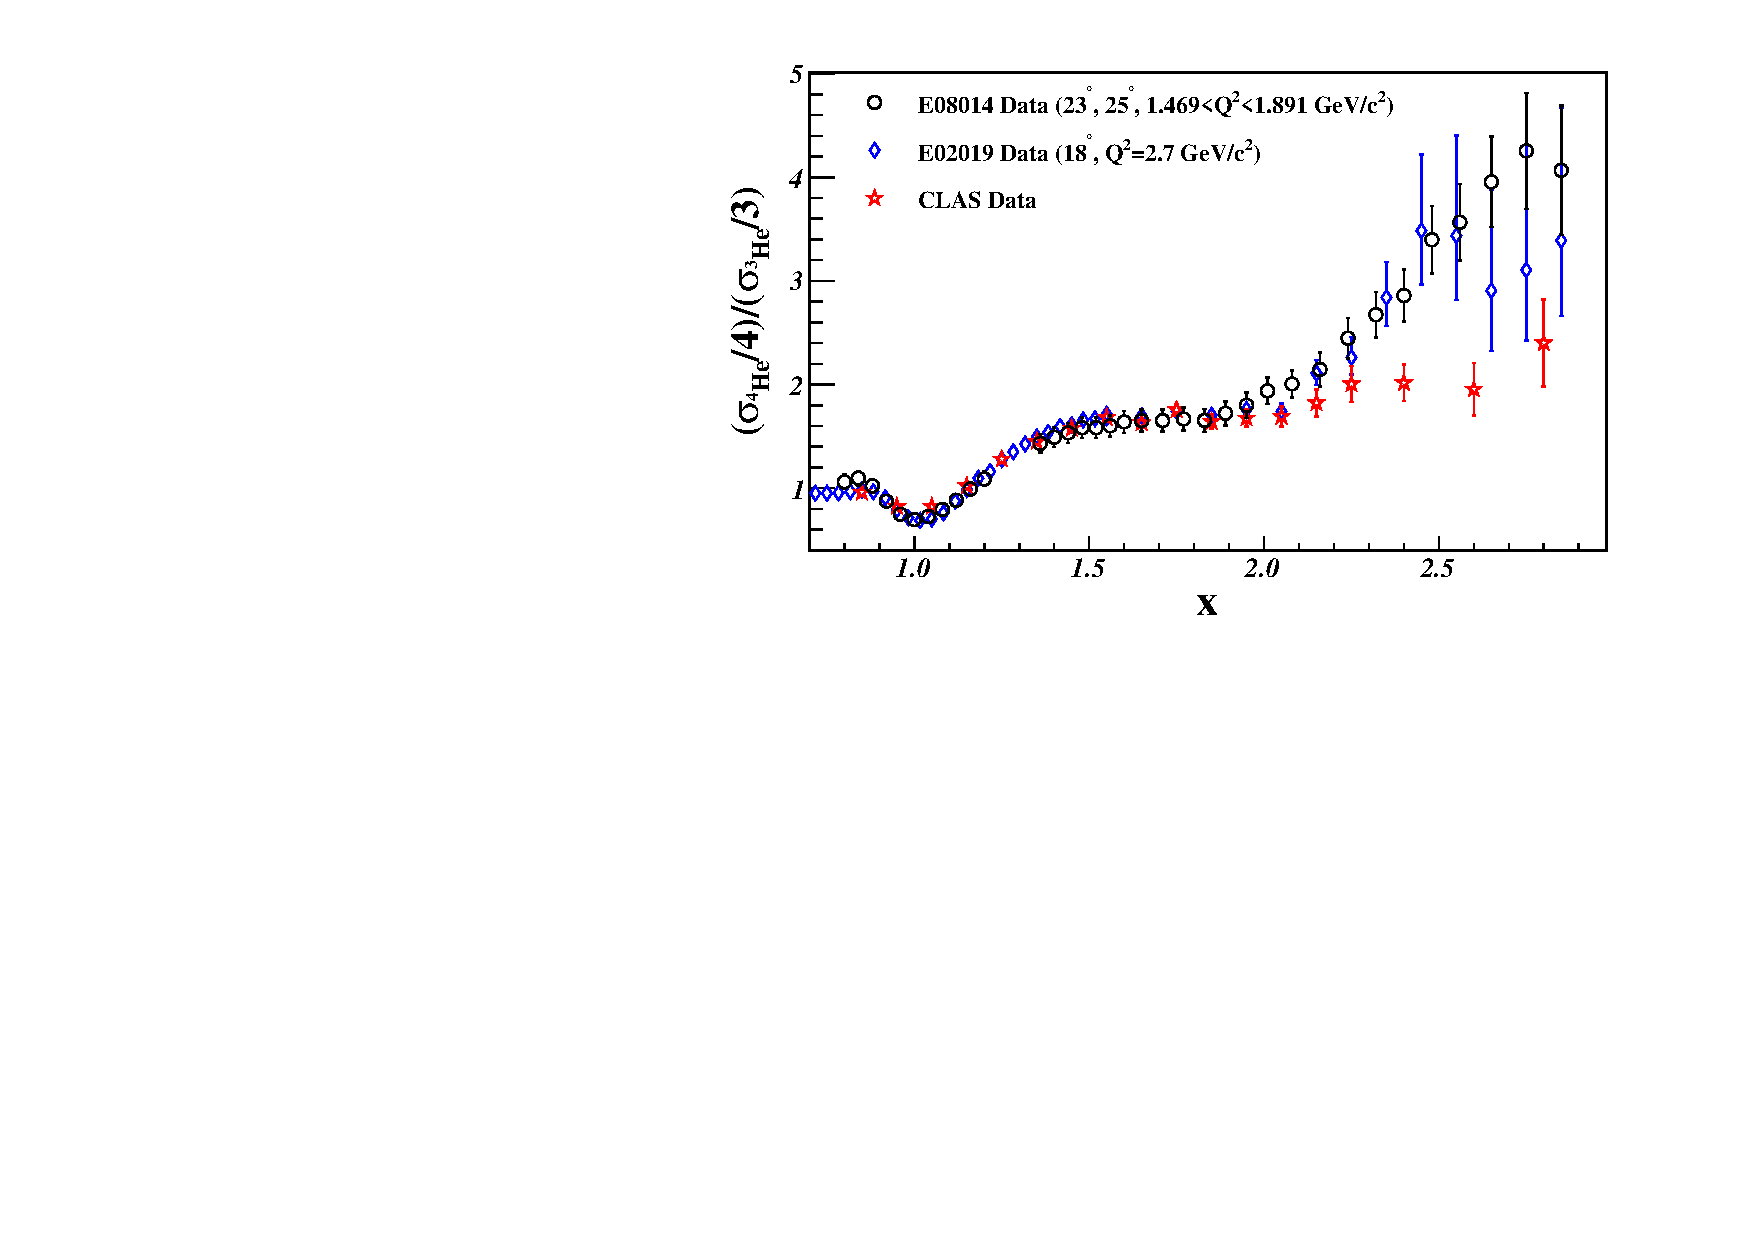
\includegraphics[width=8.5cm,angle=0]{He4_He3_XS_Ratio.pdf}
		\end{center}
		\vspace*{-5mm}
		\caption{(Color online) The $^4$He/$^3$He cross section ratio for $Q^2>1.4$~GeV$^2$ (23$^o$ and 25$^o$ scattering),
                  along with results from CLAS~\cite{PhysRevLett.96.082501} and Hall C (E02-019)~\cite{fomin2012}. The error bars include
                  statistical and systematic uncertainties; the global 5\% normalization uncertainty is not shown.}
		\label{fig:ratios_highqsq}
		\end{figure}

Figure~\ref{fig:ratios_highqsq} presents the $^4$He/$^3$He cross section ratio for our $Q^2 > 1.4$~GeV$^2$
data. In the 2N-SRC region, our data are in good agreement with the CLAS~\cite{PhysRevLett.96.082501} and
E02-019~\cite{fomin2012} results, revealing a plateau for $1.5 < x < 2$. At $x>2$, our
ratios are significantly larger than the CLAS data, but consistent within uncertainties with the E02-019
results. This is consistent with the explanation provided in a recent comment~\cite{Higinbotham:2014xna}
which concluded that the observed plateau was likely the result of large bin-migration effects resulting from
the limited CLAS momentum resolution.

While the rise in the ratio above $x=2$ indicates contributions beyond 2N-SRCs, we do not observe the 3N-SRC
plateau expected in the naive SRC model. In this model, the prediction of scaling as an indication of SRC
dominance is a simple and robust way to test for 2N-SRCs, but it is less clear how well it can indicate the
presence of 3N-SRCs. For 2N-SRCs, one can predict \textit{a priori} where the plateau should be observed
since for a given $Q^2$ value, $x$ can be chosen to require a minimum nucleon momentum above the Fermi
momentum, strongly suppressing single-particle contributions. It is not clear what values of $x$ and $Q^2$
are required to suppress 2N-SRC contributions well enough to isolate 3N-SRCs; much larger $Q^2$ values may
be required to isolate 3N-SRCs and see analogous plateaus at $x>2.5$.

                \begin{figure}[!ht]
		\begin{center}
		  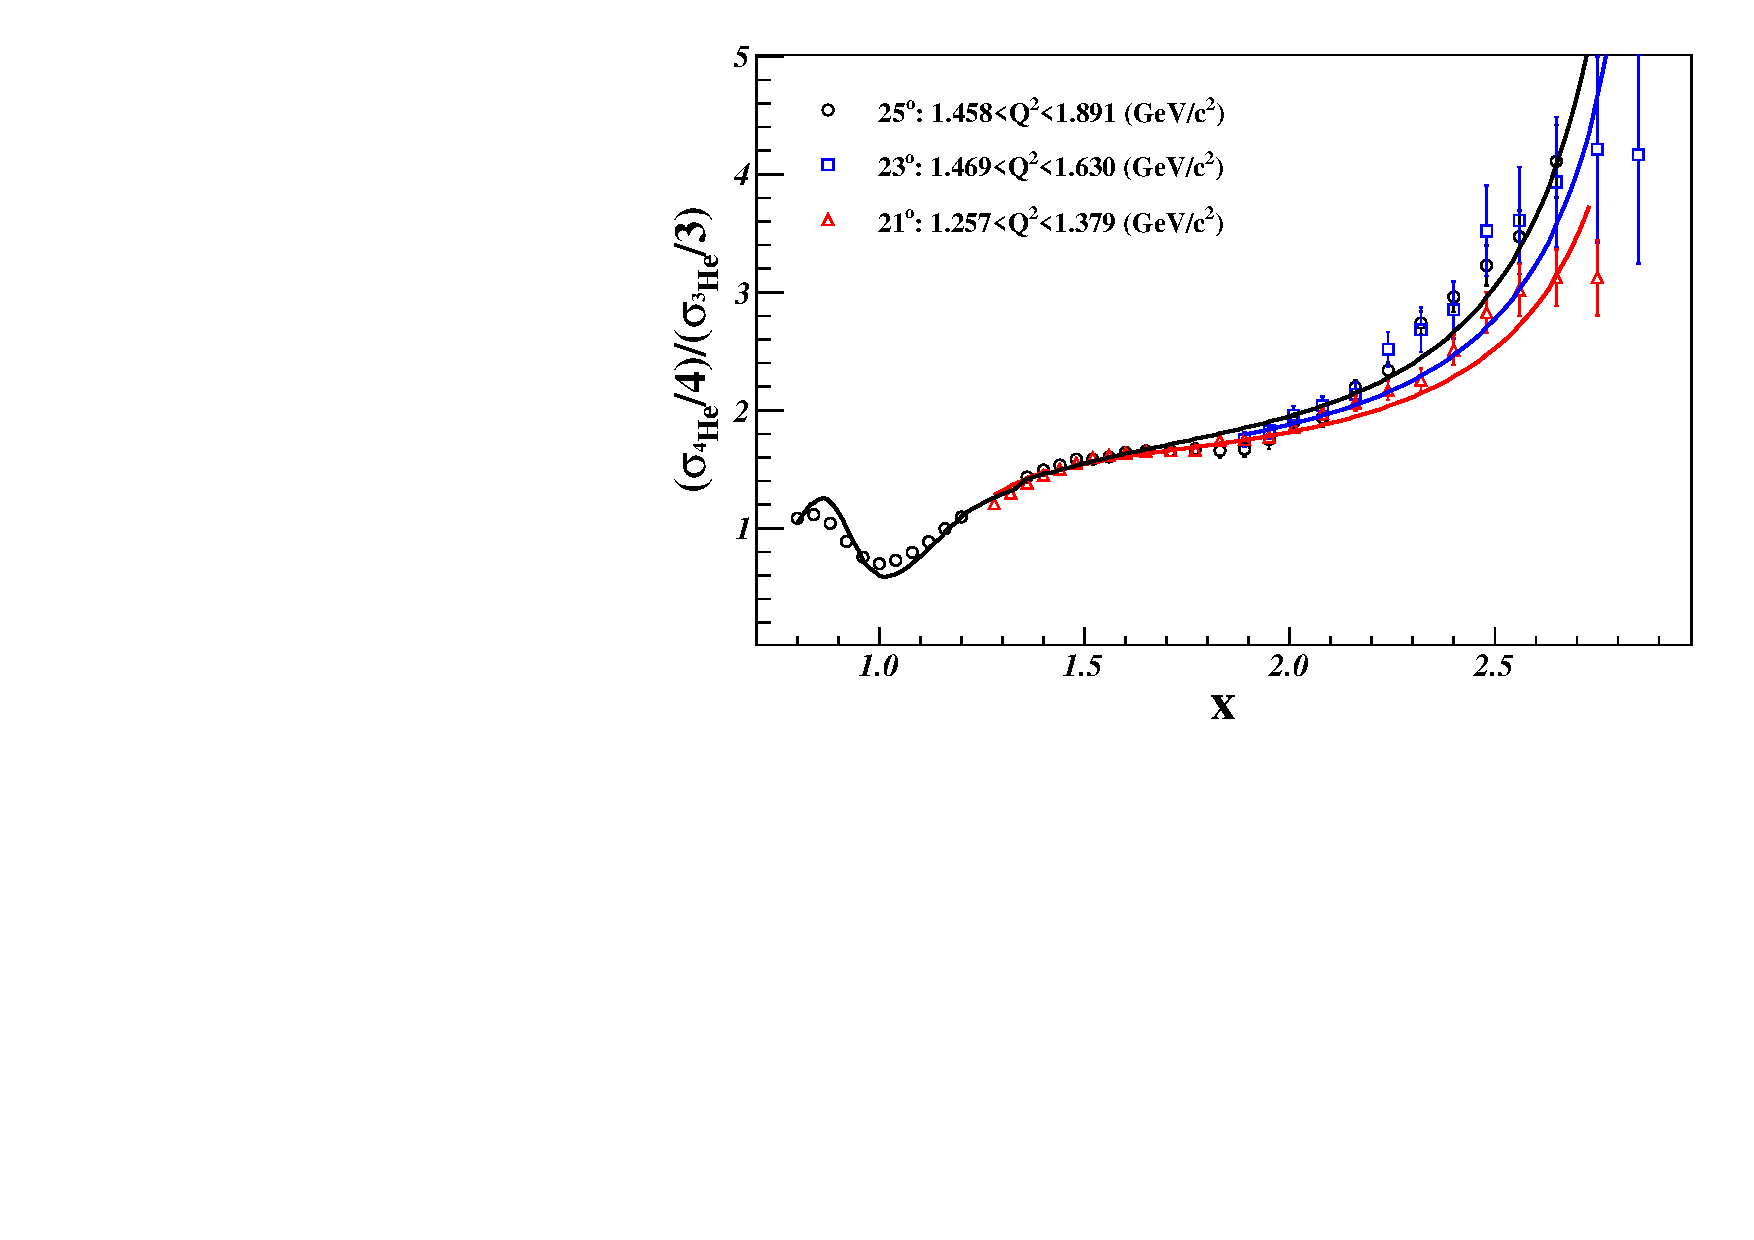
\includegraphics[width=8.5cm,angle=0]{He4_He3_XS_Ratio_MC}
                  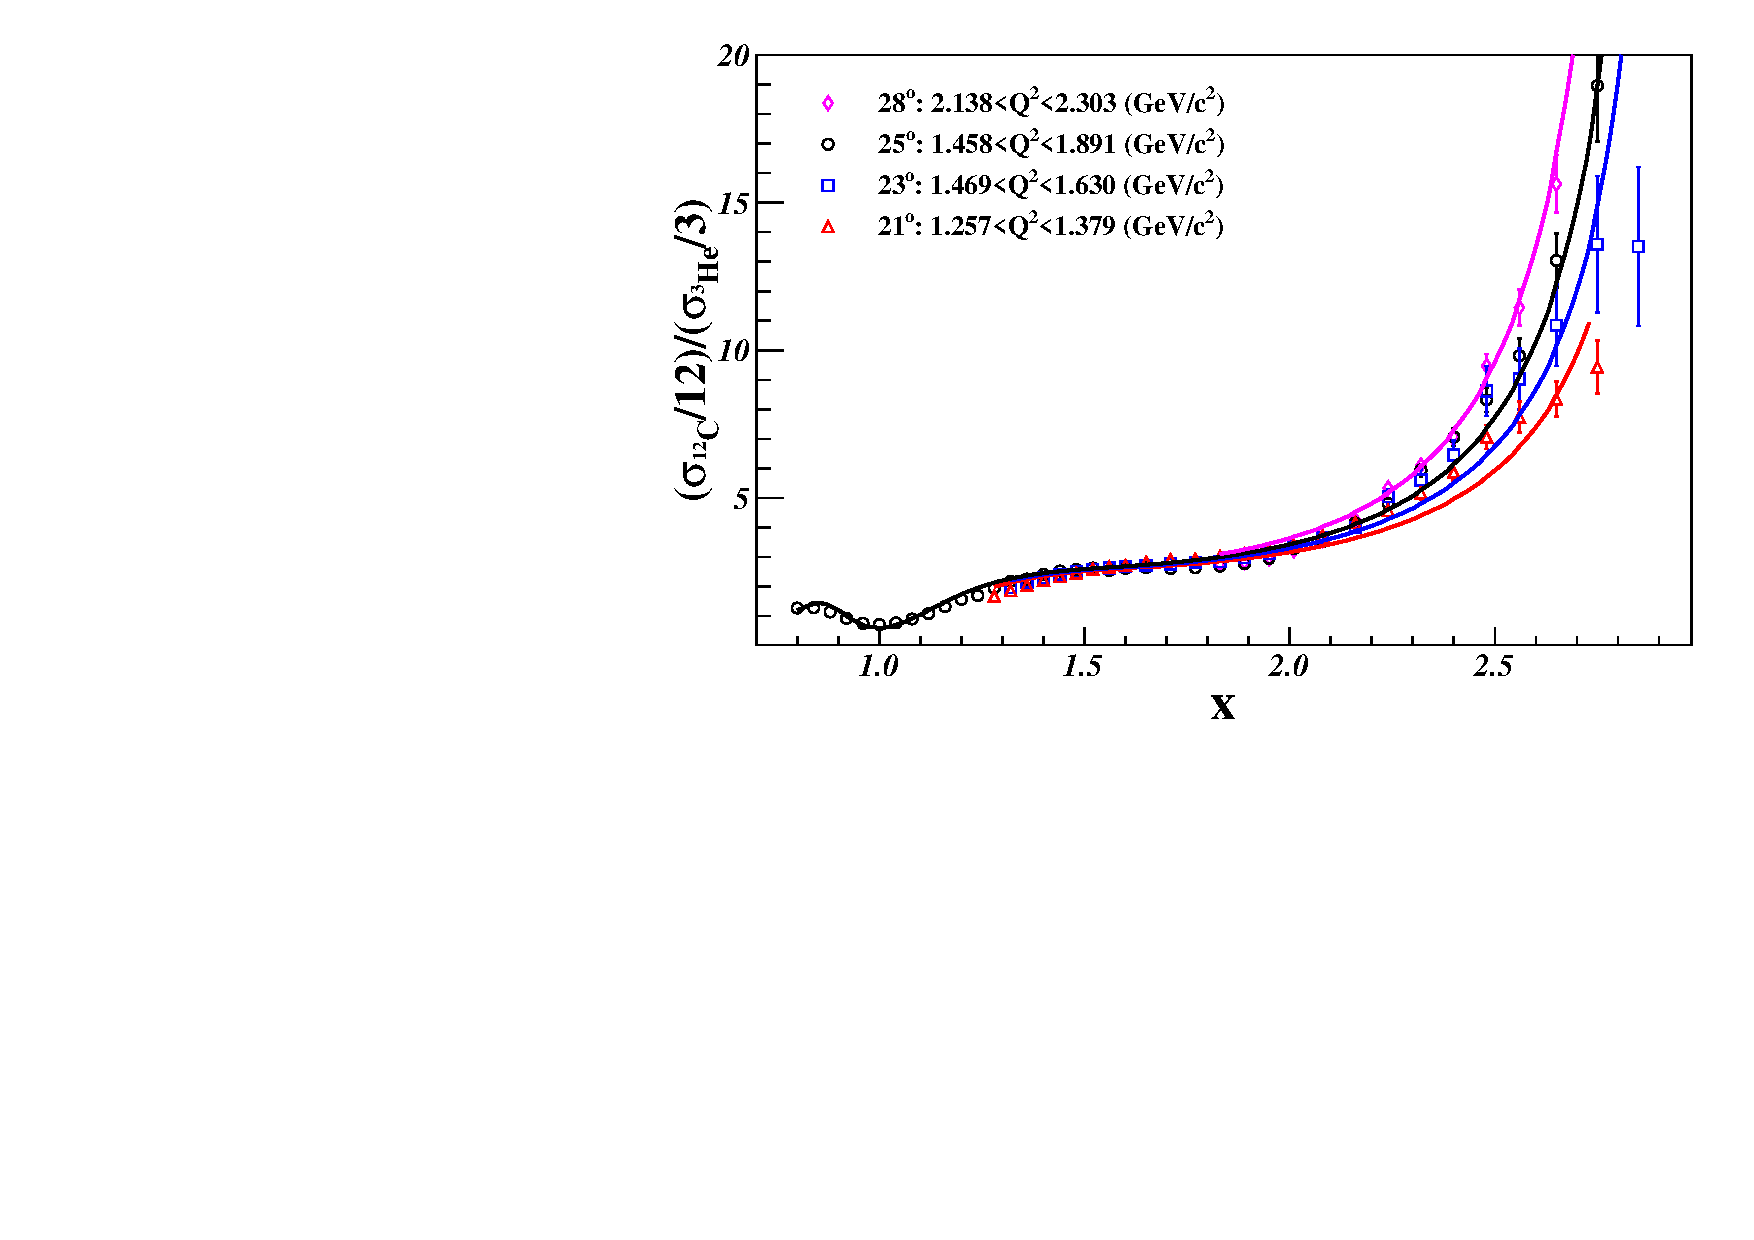
\includegraphics[width=8.5cm,angle=0]{C12_He3_XS_Ratio_MC}
		\end{center}
		\vspace*{-5mm}
		\caption{(Color online) The $^4$He/$^3$He (top) and $^{12}$C/$^3$He (bottom) cross section ratios for all angles, 
		  along with results from CLAS~\cite{PhysRevLett.96.082501} and Hall C (E02-019)~\cite{fomin2012} measurements. The solid lines
                  correspond to a simple cross section model based on parameterized momentum distributions.}
		\label{fig:ratios_allqsq}
		\end{figure}

For 2N-SRCs, the plateau must eventually disappear as the deuteron cross section falls to zero for $ x \to
M_D / M_p\approx 2$, causing the A/$^2$H ratio to rise sharply to infinity. Both the previous high-$Q^2$
deuterium data and our simple cross section model, based on a parameterization of the nulcon momentum
distribution in the nucleus, show that the
sharp drop of the deuteron cross section does not occur until $x \approx 1.9$, resulting in a clear plateau
for $1.5 < x < 1.9$. For $^3$He, our cross section model shows a similar falloff of the $^3$He cross section
starting near $x \approx 2.5$, thus yielding a rise in the A/$^3$He ratio that sets in at much lower $x$
values. This rapid rise in the A/$^3$He ratio as one approaches the $^3$He kinematic threshold shifts to
lower $x$ as $Q^2$ increases, as seen in both the data and model in Fig~\ref{fig:ratios_allqsq}. So while
the plateau is expected to set in at lower $x$ values as $Q^2$ increases, as seen in the 2N-SRC
region~\cite{ SLAC_Measurement_PRC.48.2451, PhysRevLett.96.082501}, the large-$x$ breakdown also shifts to
lower $x$ values. Thus, it is not clear whether higher $Q^2$ measurements will yield a clean way to isolate
and study 3N-SRCs.

                \begin{figure}[!ht]
		\begin{center}
		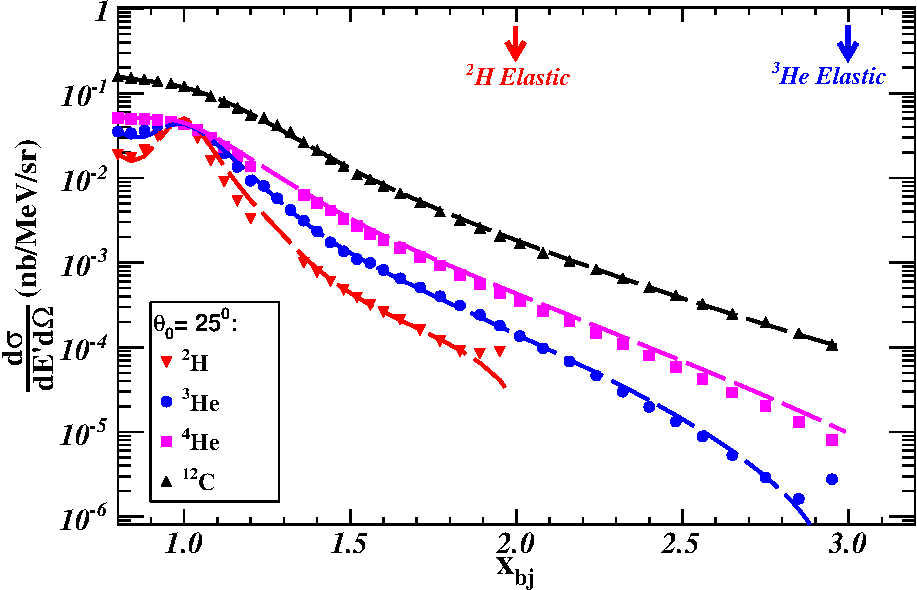
\includegraphics[width=8.5cm,angle=0]{Plot_XS_25_MC}
		\end{center}
		\vspace*{-5mm}
		\caption{(Color online) Cross sections of $^2$H, $^3$He, $^4$He and $^{12}$C at $25^{\circ}$. The uncertainties include statistical and
		systematic uncertainties. The normalization uncertainties, ranging from 2-5\%, are not shown.}
		\label{xs}
		\end{figure}

The absolute cross sections for scattering from $^{3}$He, $^{4}$He and $^{12}$C at a scattering angle of
$25^{\circ}$ are shown in Fig.~\ref{xs}. The $^3$He cross section falls more rapidly than the other nuclei
for $x>2.5$, yielding the rise in the $^4$He/$^3$He ratios discussed above. In the naive SRC model, it is
assumed that the high-$x$ cross section comes from the contributions of \textit{stationary} 2N- and 3N-SRCs.
The prediction of scaling in this model breaks down due to the difference between stationary SRC in $^2$H
(or $^3$He) and moving SRCs in heavier nuclei. For the most recent extraction of 2N-SRCs from the A/$^2$H
ratios~\cite{fomin2012}, the effect of the 2N-SRC motion in heavier nuclei was estimated and found to give a
small enhancement of the ratio in the plateau region, with little distortion of the shape until $x >
1.9$~\cite{fomin2012} where the ratio rises rapidly to infinity. For 3N-SRCs, motion of the correlations
produces a similar rise which begins well before the kinematic limit at $x \approx 3$. This picture is also
consistent with the observation that the $x > 2.5$ increase in the ratio is larger for $^{12}$C/$^3$He.
However, a clear interpretation of the large $x$ behavior of $^{12}$C/$^3$He is more difficult. At very large
$x$ values, where the cross section drops rapidly, the data are very sensitive to the spectrometer resolution.
When comparing two thin targets, or two extended targets, the acceptance and resolution effects cancel, 
stronly suppressing such effects in the target ratios. However, in the ratio of $^{12}$C/$^3$He, the variation
of the resolution with target length and the possible impact of correlations between the scattering angles and
the reconstructed target position can yield different resolution effects for the two targets. So while the
rise in the $^{12}$C/$^3$He can be explained by the comparison of moving 3N-SRCs to stationary ones, there
can be additional effects due to the difference in resolution between the foil targets and the 20cm ${3,4}$He
targets.


%\textit{impact of isospin dependence?}.


%In attempting to isolate 3N-SRC contributions, the situation is less straightforward. Both 2N and 3N SRCs yield contributions to the high-momentum
%tail. The fact that we do not see significant deviations from the 2N-SRC picture for $1.5<x<2$ suggests that the 3N-SRC contributions are generally
%much smaller. Unlike the case for 2N-SRCs, where $k>k_F$ suppresses single particle strength, there is not a clear way to define a threshold in $x$
%that will sufficiently suppress 2N contributions.  Approaching the kinematic limit at $x \approx 3$, the $^3$He cross section falls to zero and the
%ratio must go to infinity. However, while this occurs in a vary narrow $x$ window for the A/$^2$H ratios, the rise occurs over a larger range in $x$
%in this case.

%Thus, it is not clear that there will be a significant window in $x$ where one would expect to see a plateau, especially at the relatively modest
%$Q^2$ values measured here. In the present experiment, we observe a small but noticeable $Q^2$ dependence, in particular for $x \gtorder 2.5$. This
%is also observed in our simple $y$-scaling cross section model, and does not occur in the $^{12}$C/$^3$He ratio, indicating that it is the $x$
%dependence of the falloff of the $^3$He cross section as $x \to 3$ that is varying strongly with $Q^2$. Larger $Q^2$ values may be required to
%observe a $Q^2$-independent behavior of the ratios with $x$, which may allow us to isolate 3N-SRC contributions.



%\textit{Figure with A/2H ratios up to $x=2$, table with $a_2$ results for $A=3$, 4, 12, 48?}


%JRA Notes:
%0) Can we look at A/D ratios vs. Q^2 for our cross section model? Impact of x-->2 in 2H? Where does A/D rise up for x-->2?
%1) x-->3 has may have larger missing energy (plus, smaller energy step from x=1 to 2 to 3, so may fall to zero over wider range.
%2) $Q^2$ dependence of $x \to 3$ ratios in general agreement with what we observe in our cross section model. Suggests that the cross
%section falloff as we approach the kinematic threshold is large

%results
            \begin{figure}[!ht]
		\begin{center}
		  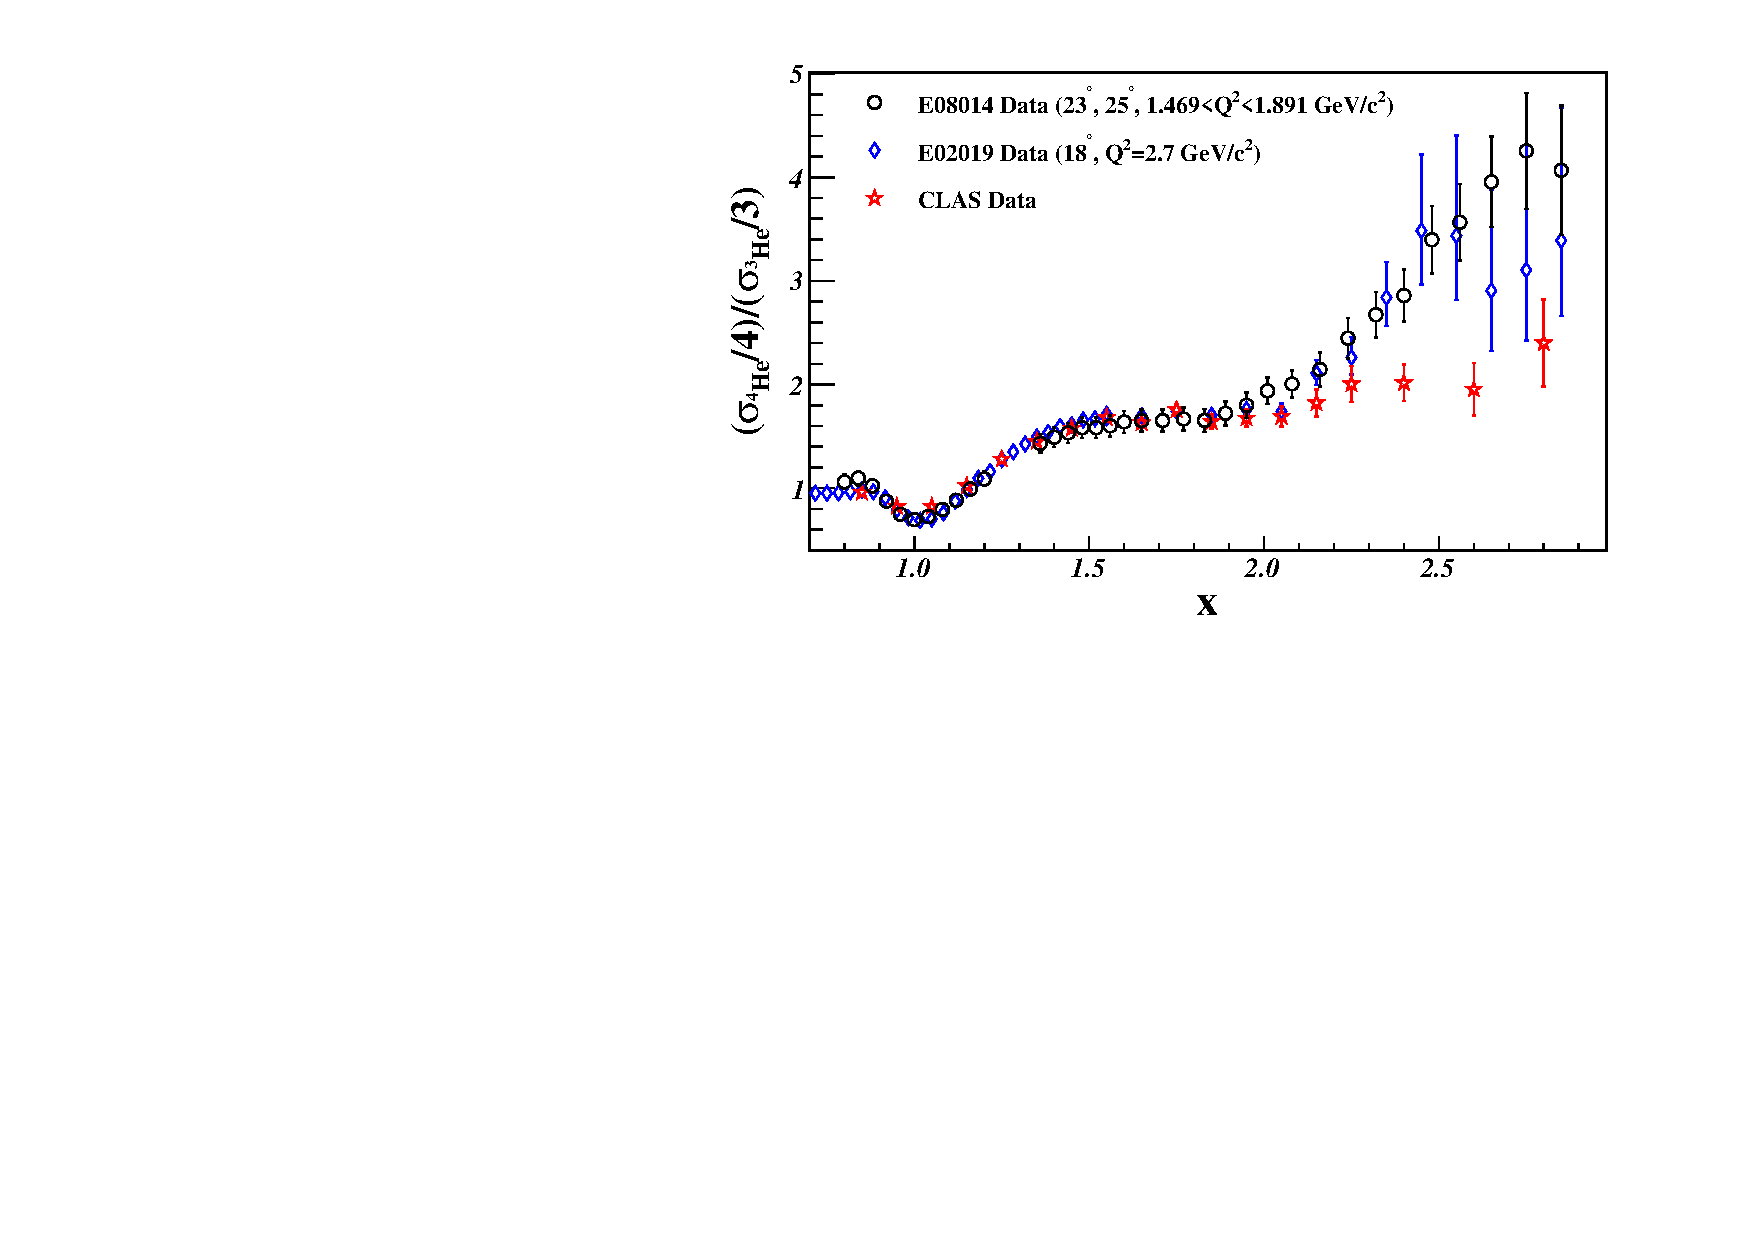
\includegraphics[width=8.5cm,angle=0]{He4_He3_XS_Ratio.pdf}
		\end{center}
		\vspace*{-5mm}
		\caption{(Color online) The $^4$He/$^3$He cross section ratio for $Q^2>1.4$~GeV$^2$ (23$^o$ and 25$^o$ scattering),
                  along with results from CLAS~\cite{PhysRevLett.96.082501} and Hall C (E02-019)~\cite{fomin2012}. The error bars include
                  statistical and systematic uncertainties; the global 5\% normalization uncertainty is not shown.}
		\label{fig:ratios_highqsq}
		\end{figure}

Figure~\ref{fig:ratios_highqsq} presents the $^4$He/$^3$He cross section ratio for our $Q^2 > 1.4$~GeV$^2$
data. In the 2N-SRC region, our data are in good agreement with the CLAS~\cite{PhysRevLett.96.082501} and
E02-019~\cite{fomin2012} results, revealing a plateau for $1.5 < x < 2$. At $x>2$, our
ratios are significantly larger than the CLAS data, but consistent within uncertainties with the E02-019
results. This is consistent with the explanation provided in a recent comment~\cite{Higinbotham:2014xna}
which concluded that the observed plateau was likely the result of large bin-migration effects resulting from
the limited CLAS momentum resolution.

While the rise in the ratio above $x=2$ indicates contributions beyond 2N-SRCs, we do not observe the 3N-SRC
plateau expected in the naive SRC model. In this model, the prediction of scaling as an indication of SRC
dominance is a simple and robust way to test for 2N-SRCs, but it is less clear how well it can indicate the
presence of 3N-SRCs. For 2N-SRCs, one can predict \textit{a priori} where the plateau should be observed
since for a given $Q^2$ value, $x$ can be chosen to require a minimum nucleon momentum above the Fermi
momentum, strongly suppressing single-particle contributions. It is not clear what values of $x$ and $Q^2$
are required to suppress 2N-SRC contributions well enough to isolate 3N-SRCs; much larger $Q^2$ values may
be required to isolate 3N-SRCs and see analogous plateaus at $x>2.5$.

                \begin{figure}[!ht]
		\begin{center}
		  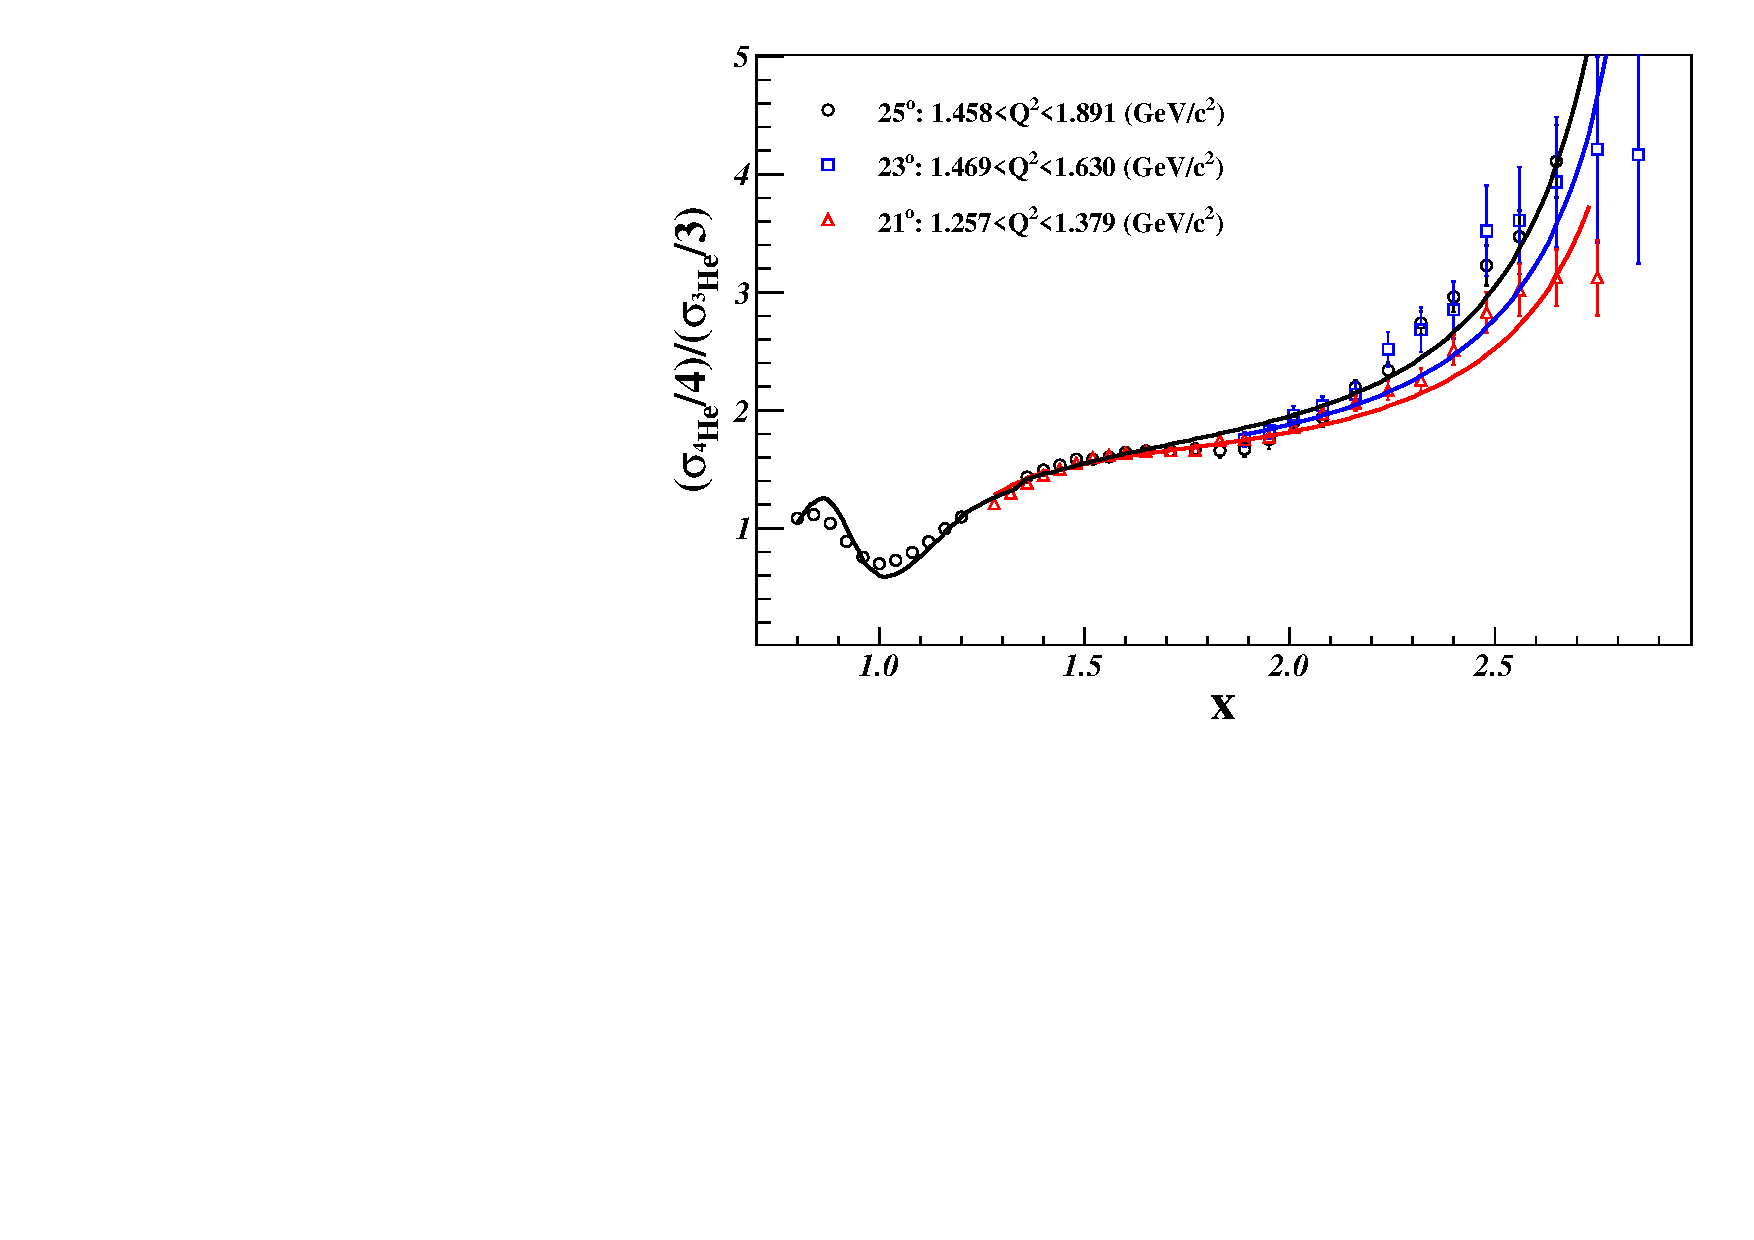
\includegraphics[width=8.5cm,angle=0]{He4_He3_XS_Ratio_MC}
                  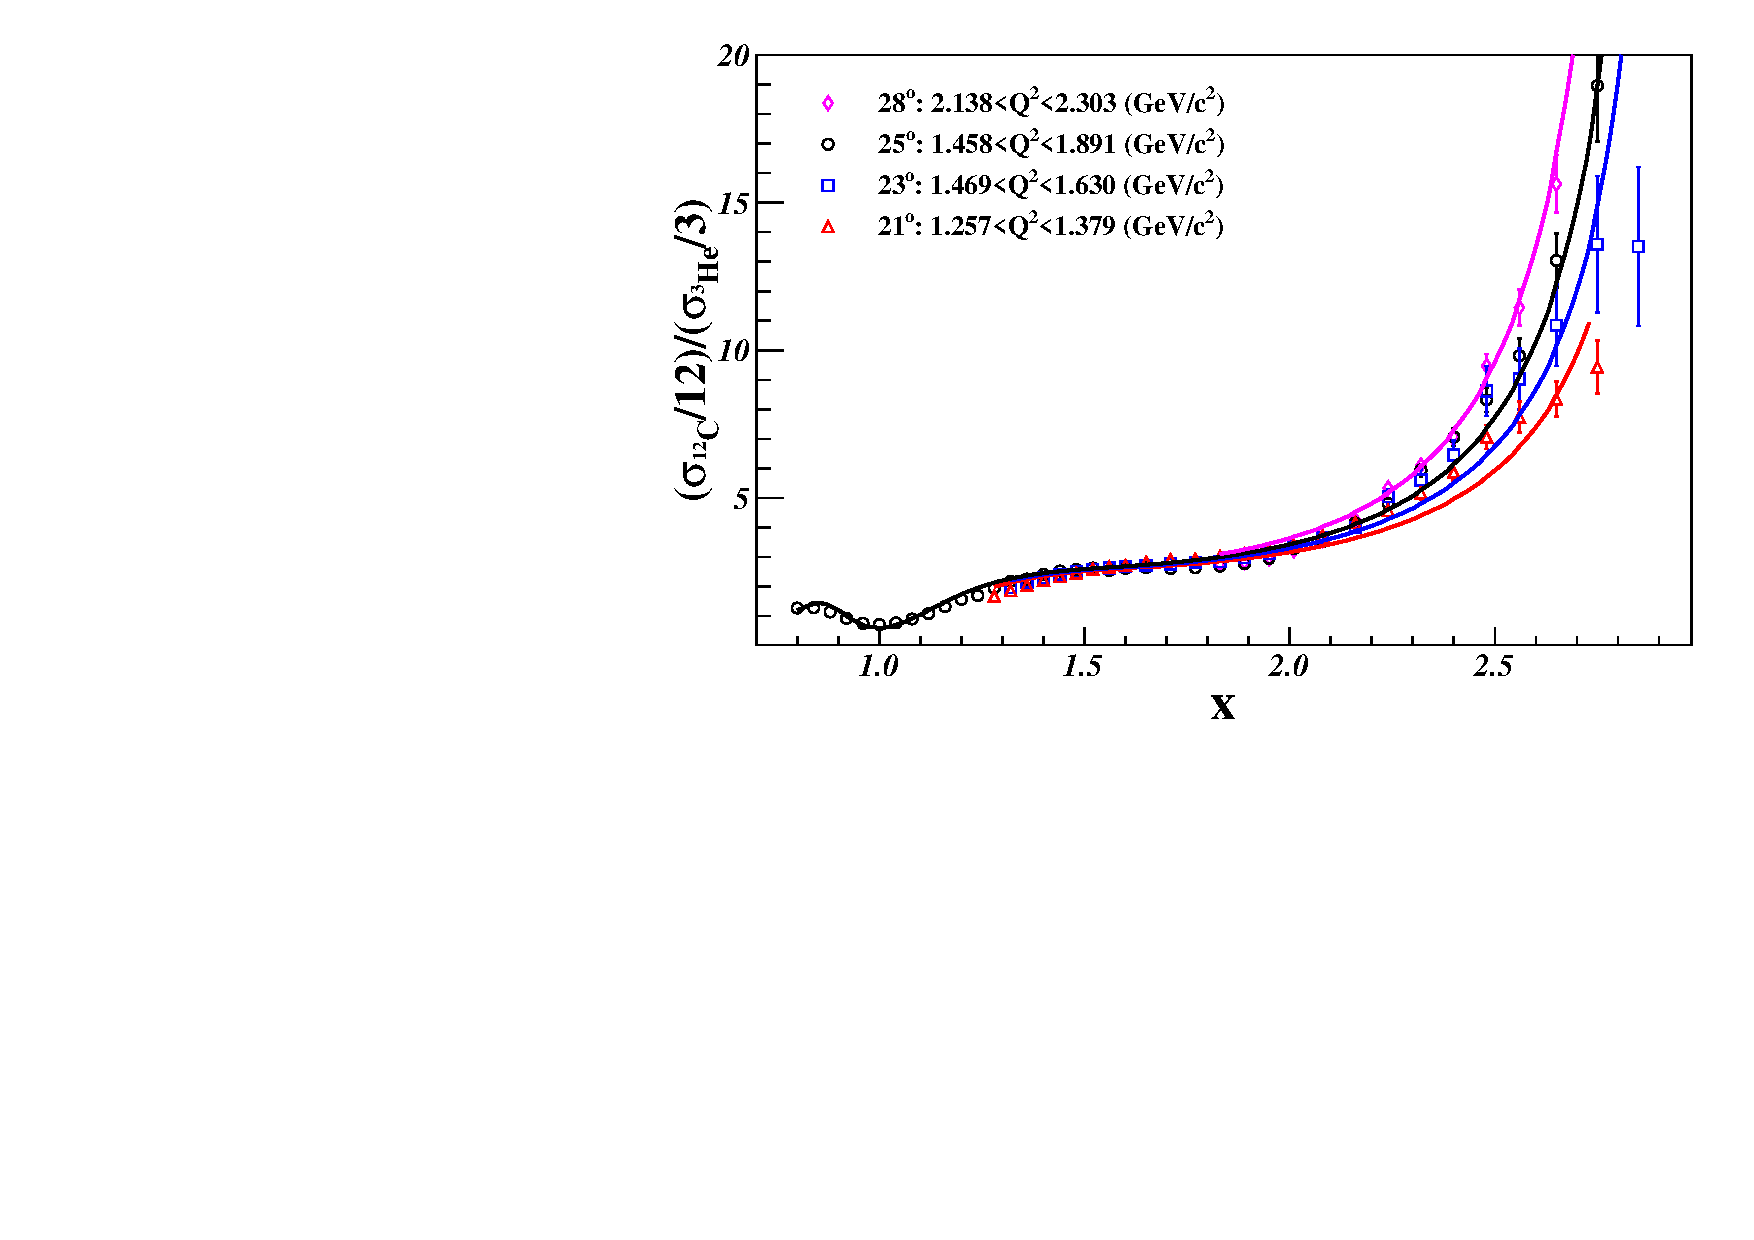
\includegraphics[width=8.5cm,angle=0]{C12_He3_XS_Ratio_MC}
		\end{center}
		\vspace*{-5mm}
		\caption{(Color online) The $^4$He/$^3$He (top) and $^{12}$C/$^3$He (bottom) cross section ratios for all angles, 
		  along with results from CLAS~\cite{PhysRevLett.96.082501} and Hall C (E02-019)~\cite{fomin2012} measurements. The solid lines
                  correspond to a simple cross section model based on parameterized momentum distributions.}
		\label{fig:ratios_allqsq}
		\end{figure}

For 2N-SRCs, the plateau must eventually disappear as the deuteron cross section falls to zero for $ x \to
M_D / M_p\approx 2$, causing the A/$^2$H ratio to rise sharply to infinity. Both the previous high-$Q^2$
deuterium data and our simple cross section model, based on a parameterization of the nulcon momentum
distribution in the nucleus, show that the
sharp drop of the deuteron cross section does not occur until $x \approx 1.9$, resulting in a clear plateau
for $1.5 < x < 1.9$. For $^3$He, our cross section model shows a similar falloff of the $^3$He cross section
starting near $x \approx 2.5$, thus yielding a rise in the A/$^3$He ratio that sets in at much lower $x$
values. This rapid rise in the A/$^3$He ratio as one approaches the $^3$He kinematic threshold shifts to
lower $x$ as $Q^2$ increases, as seen in both the data and model in Fig~\ref{fig:ratios_allqsq}. So while
the plateau is expected to set in at lower $x$ values as $Q^2$ increases, as seen in the 2N-SRC
region~\cite{ SLAC_Measurement_PRC.48.2451, PhysRevLett.96.082501}, the large-$x$ breakdown also shifts to
lower $x$ values. Thus, it is not clear whether higher $Q^2$ measurements will yield a clean way to isolate
and study 3N-SRCs.

                \begin{figure}[!ht]
		\begin{center}
		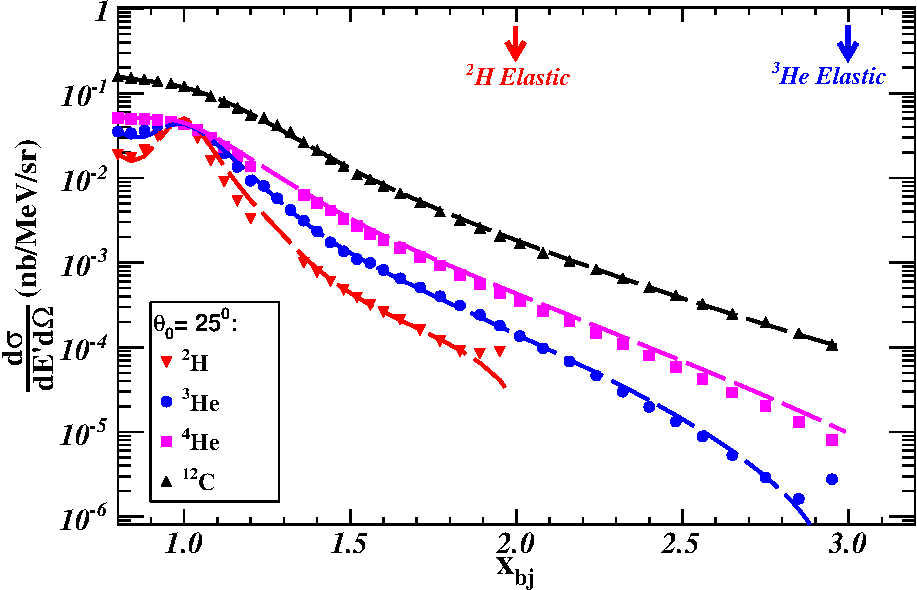
\includegraphics[width=8.5cm,angle=0]{Plot_XS_25_MC}
		\end{center}
		\vspace*{-5mm}
		\caption{(Color online) Cross sections of $^2$H, $^3$He, $^4$He and $^{12}$C at $25^{\circ}$. The uncertainties include statistical and
		systematic uncertainties. The normalization uncertainties, ranging from 2-5\%, are not shown.}
		\label{xs}
		\end{figure}

The absolute cross sections for scattering from $^{3}$He, $^{4}$He and $^{12}$C at a scattering angle of
$25^{\circ}$ are shown in Fig.~\ref{xs}. The $^3$He cross section falls more rapidly than the other nuclei
for $x>2.5$, yielding the rise in the $^4$He/$^3$He ratios discussed above. In the naive SRC model, it is
assumed that the high-$x$ cross section comes from the contributions of \textit{stationary} 2N- and 3N-SRCs.
The prediction of scaling in this model breaks down due to the difference between stationary SRC in $^2$H
(or $^3$He) and moving SRCs in heavier nuclei. For the most recent extraction of 2N-SRCs from the A/$^2$H
ratios~\cite{fomin2012}, the effect of the 2N-SRC motion in heavier nuclei was estimated and found to give a
small enhancement of the ratio in the plateau region, with little distortion of the shape until $x >
1.9$~\cite{fomin2012} where the ratio rises rapidly to infinity. For 3N-SRCs, motion of the correlations
produces a similar rise which begins well before the kinematic limit at $x \approx 3$. This picture is also
consistent with the observation that the $x > 2.5$ increase in the ratio is larger for $^{12}$C/$^3$He.
However, a clear interpretation of the large $x$ behavior of $^{12}$C/$^3$He is more difficult. At very large
$x$ values, where the cross section drops rapidly, the data are very sensitive to the spectrometer resolution.
When comparing two thin targets, or two extended targets, the acceptance and resolution effects cancel, 
stronly suppressing such effects in the target ratios. However, in the ratio of $^{12}$C/$^3$He, the variation
of the resolution with target length and the possible impact of correlations between the scattering angles and
the reconstructed target position can yield different resolution effects for the two targets. So while the
rise in the $^{12}$C/$^3$He can be explained by the comparison of moving 3N-SRCs to stationary ones, there
can be additional effects due to the difference in resolution between the foil targets and the 20cm ${3,4}$He
targets.


%\textit{impact of isospin dependence?}.


%In attempting to isolate 3N-SRC contributions, the situation is less straightforward. Both 2N and 3N SRCs yield contributions to the high-momentum
%tail. The fact that we do not see significant deviations from the 2N-SRC picture for $1.5<x<2$ suggests that the 3N-SRC contributions are generally
%much smaller. Unlike the case for 2N-SRCs, where $k>k_F$ suppresses single particle strength, there is not a clear way to define a threshold in $x$
%that will sufficiently suppress 2N contributions.  Approaching the kinematic limit at $x \approx 3$, the $^3$He cross section falls to zero and the
%ratio must go to infinity. However, while this occurs in a vary narrow $x$ window for the A/$^2$H ratios, the rise occurs over a larger range in $x$
%in this case.

%Thus, it is not clear that there will be a significant window in $x$ where one would expect to see a plateau, especially at the relatively modest
%$Q^2$ values measured here. In the present experiment, we observe a small but noticeable $Q^2$ dependence, in particular for $x \gtorder 2.5$. This
%is also observed in our simple $y$-scaling cross section model, and does not occur in the $^{12}$C/$^3$He ratio, indicating that it is the $x$
%dependence of the falloff of the $^3$He cross section as $x \to 3$ that is varying strongly with $Q^2$. Larger $Q^2$ values may be required to
%observe a $Q^2$-independent behavior of the ratios with $x$, which may allow us to isolate 3N-SRC contributions.



%\textit{Figure with A/2H ratios up to $x=2$, table with $a_2$ results for $A=3$, 4, 12, 48?}


%JRA Notes:
%0) Can we look at A/D ratios vs. Q^2 for our cross section model? Impact of x-->2 in 2H? Where does A/D rise up for x-->2?
%1) x-->3 has may have larger missing energy (plus, smaller energy step from x=1 to 2 to 3, so may fall to zero over wider range.
%2) $Q^2$ dependence of $x \to 3$ ratios in general agreement with what we observe in our cross section model. Suggests that the cross
%section falloff as we approach the kinematic threshold is large


%%%%%%%%%%%%%%%%%%%%%%%%%%%%%%%%%%%%%%%%%%%%%%%%%%%%%
%discussion
%	% conclusions
(Add conclusion here)

	

%%%%%%%%%%%%%%%%%%%%%%%%%%%%%%%%%%%%%%%%%%%%%%%%%%%%%
We have performed high-statistics measurements of the $^4$He/$^3$He and $^{12}$C/$^3$He cross section
ratios, confirming the results of the low-statistics measurements from Hall C~\cite{fomin2012} and showing
a clear disagreement with the CLAS data~\cite{PhysRevLett.96.082501}. This supports the idea that the CLAS
data were limited at large $x$ by bin-migration effects due to the spectrometer's modest momentum
resolution~\cite{Higinbotham:2014xna}. We do not observe the plateau predicted by the naive SRC model, but
explain why the prediction for the inclusive ratios in the 3N-SRC regime are not as robust as those for
2N-SRC. While we do not observe the predicted plateau, this does not demonstrate that 3N-SRCs are
unimportant in this region. Even if the cross section is dominated by 3N-SRCs, the inclusive scattering
ratios may not show a plateau due to the motion of the 3N-SRCs.

While the A/$^3$He ratios do not provide a direct signature of 3N-SRCs, it should still be possible to use
inclusive scattering to look for contributions of 3N configurations in nuclei. The biggest obstacle appears
to be the limited region in $x$ where the correction for the motion of any 3N-SRCs in heavy nuclei is small.
This problem can be avoided if one compares the $^3$He scattering at large $x$ with a model of the
contributions of moving 2N-SRCs in $^3$He. The contribution of 3N-SRCs would appear as an increase in the
cross section relative to what is expected when modeling scattering from $^3$He in terms of single-particle
strength and 2N-SRC contributions, including precise, quantitative corrections for the motion of the
2N-SRCs. However, because this is a comparison to theory, rather than a comparison of SRCs within two
nuclei, one can no longer rely on final-state interactions canceling in the comparison, and these effects
would have to be modeled.

It will be important for such comparisons to be performed over a range of $Q^2$, making the data to be taken
at Jefferson Lab after the energy upgrade important for such studies~\cite{e1206105}. In addition,
comparisons of scattering from $^3$He and $^3$H at large $x$~\cite{e1211112} allow for comparison of the
isospin structure in the high-momentum components of the $^3$H and $^3$He nucleon momentum distributions. If
only 2N-SRCs contribute at large momenta, then the observed n-p pair dominance will yield nearly identical
cross sections for the $x>2$ region as well, while contributions from 3N-SRCs need not be isospin independent.

\begin{acknowledgments}

We would like to acknowledge the outstanding support from the Jefferson Lab Hall A technical staff and the
JLab target group. This work was supported in part by the DOE Office of Science, Office of Nuclear Physics,
contract DE-FG02-96ER40950, under which JSA, LLC operates JLab, DOE contracts DE-AC02-06CH11357,
DE-AC05-06OR23177, the National Science Foundation, and the UK Science and Technology Facilities Council
(ST/J000175/1,ST/G008604/1).

\end{acknowledgments}

%\bibliographystyle{apsrev4-1}
\bibliographystyle{h-physrev3.bst}
\bibliography{e08014}

\end{document}
